\chapter{Results}
\label{Results}
In this chapter, we go over the data set we have built from our IoT test bed and present graphs from that data set. This chapter starts with the effects of changing the smart plug that the device connects to in section \ref{swappingSwitch}. Then section \ref{wholeDB} covers the protocol spread over the whole database. The next two subsections \ref{Smart Speakers} and \ref{Streaming Devices} covers smart speakers and streaming devices while idle, in use, and during first boot, including other intersting results if any. Sections \ref{sumPowerGraph} and\ref{sumPowerGraphWithNoise} covers the summed power graphs that simulate a shared powerline with and without noise. Finally this chapter concludes with a comparison between smart speakers in section \ref{smartSpeakerComparisonSection}.

Sections \ref{Whole Database}, \ref{smartSpeakerResults}, and \ref{Streaming Devices} are covered in Ryan Frawley's paper\cite{frawley_2018} and are paraphrased with no further discussion in section \ref{Discussion}. Frawley's paper contains a more in-depth analysis in those sections and include GeoIP information that highlights the spread of locations the database and each device communicates with the most.

When obtaining data, most of the packets are encrypted, so the data we present focuses on metadata such as size, protocol, source IP, dest IP. For power analysis, we only use the power used at each second.

\section{Swapping the Power Switch}
\label{swappingSwitch}
We wanted to check if the smart switches were consistent between devices. To do so, we swapped various devices with various power switches and checked to see if the idle power was still the same. After doing so multiple times with various devices, we found no change when swapping the switches. One example is shown in figure  \ref{fig:switchEchoEufyPlug} where we plugged the Echo Dot 1 into the Eufy
Genie 1's corresponding Wemo smart switch and vice versa. After starting restarting up from power on, the Eufy Genie's power reads the same as the Echo Dot had previously read and vice versa.

\begin{figure}[H]
    \centering
    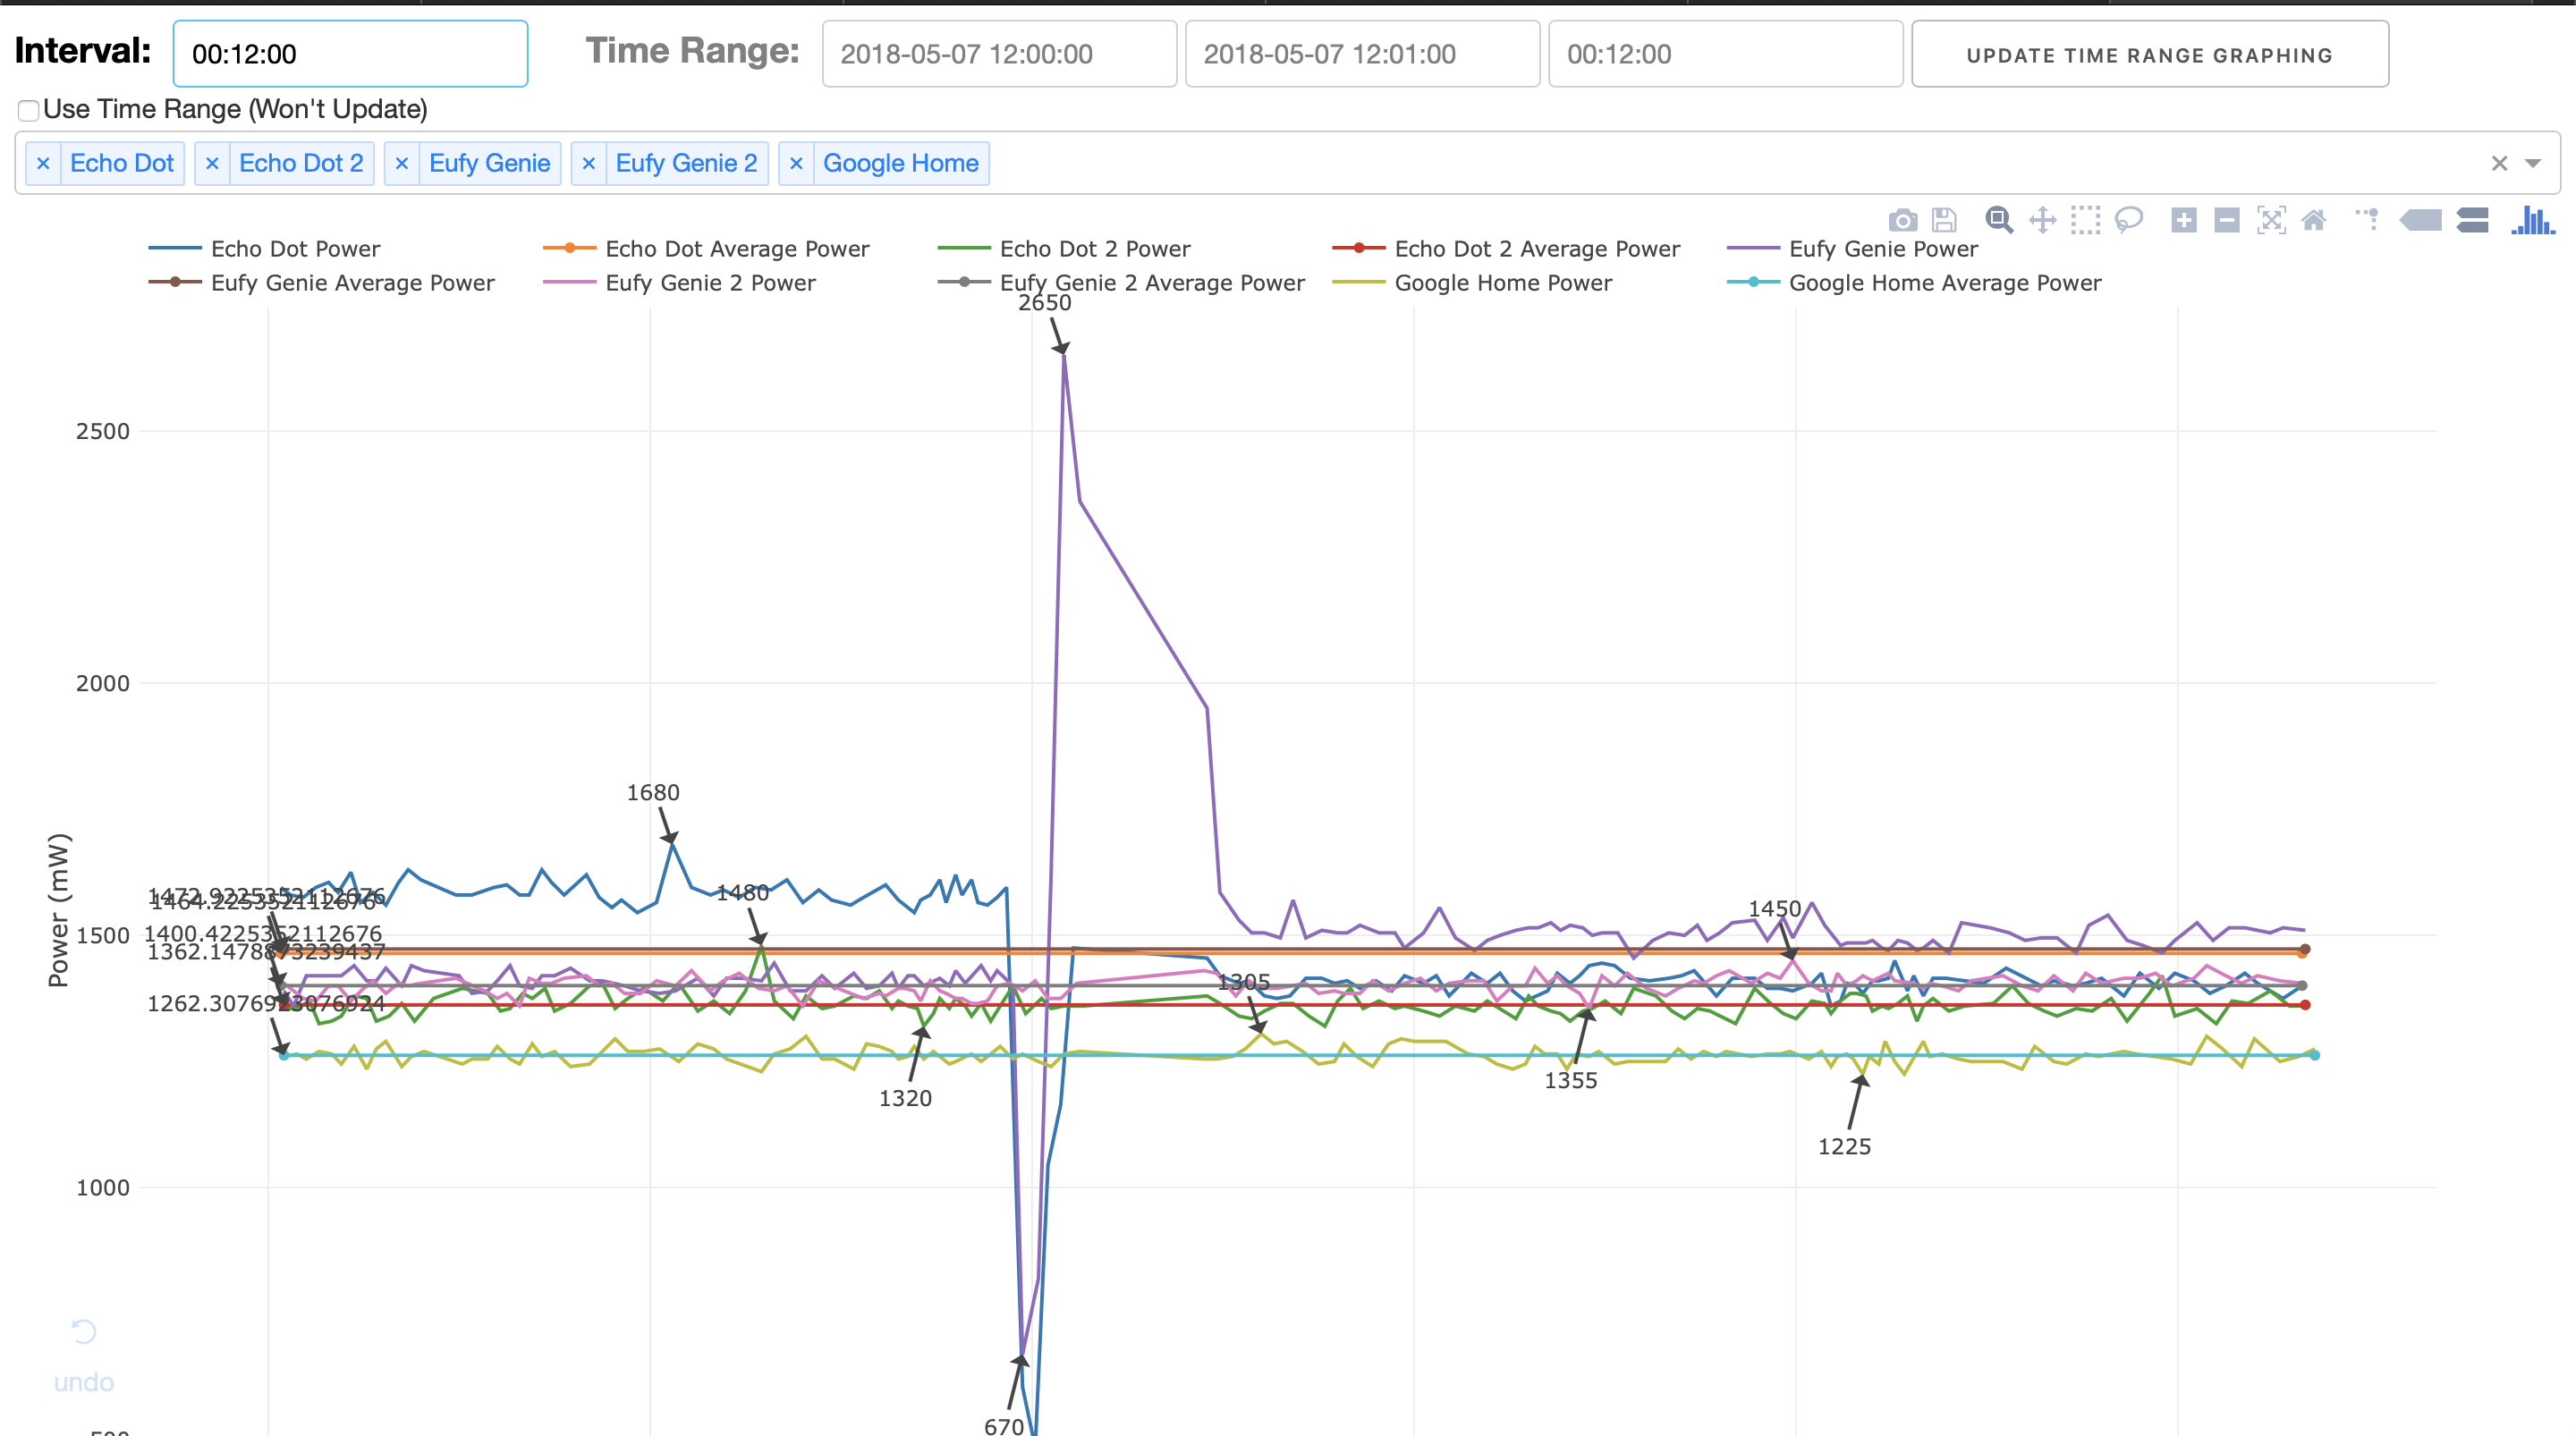
\includegraphics[width=1\textwidth]{figures/switchEchoEufyPlug.png}
    \caption{Switching the Echo Dot 1 and Eufy Genie 1's smart switch}
    \label{fig:switchEchoEufyPlug}
\end{figure}

\section{Whole Database}
\label{wholeDB}
When examining the whole database, most of the traffic goes through TCP so that communication can be more reliable. Then UDP comes next as it is beneficial for streaming and communication services, then finally IGMP and everything else. The spread of protocols can be shown in figure \ref{fig:tcpudp}.

\label{Whole Database}
\begin{figure}[H]
  \centering
    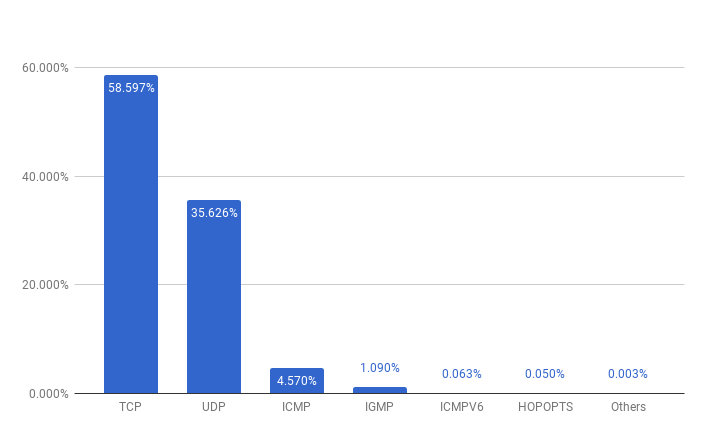
\includegraphics[width=1\textwidth]{tcpudp}
  \caption{Internet and Transport Layer Protocols in Database}
  \label{fig:tcpudp}
\end{figure}

\section{Smart Speakers}
\label{smartSpeakerResults}
\subsection{Google Home Mini}
The Google home mini's idle traffic broadcasts SSDP (Simple Service Discovery Protocol) packets once every minute. The SSDP packets are a discovery request packet for every IoT device on the network that supports UPnP (Universal Plug and Play). At which point devices such as the Echo Dot, Samsung TV, streaming devices, and the Chromebook would respond with information about themselves in a .xml file. This XML file contains details regarding the device operating system and more. Google also sends encrypted TCP packets to Google every 10 minutes. The Google Home Mini's idle traffic is shown in figure \ref{fig:home}. The high peaks are the encrypted TCP packets, and the smaller spikes are the SSDP/UPnP packets.

\begin{figure}[H]
  \centering
    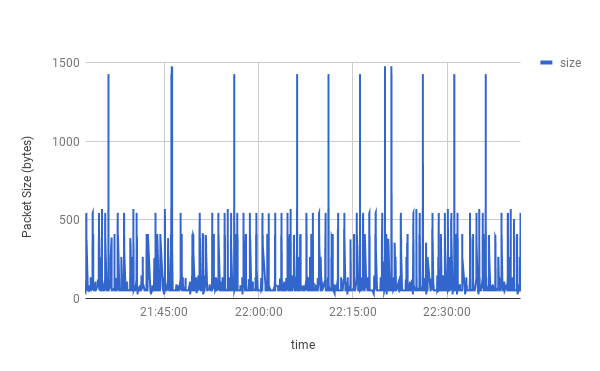
\includegraphics[width=0.9\textwidth]{home1hr}
  \caption{Idle Traffic of Google Home Over 1 Hour Period}
  \label{fig:home}
\end{figure}

A graph of the Google Home Mini is shown in the figure \ref{fig:homequery}. The Google Home Mini is first asked for the news and then told to stop. After waiting for 40 minutes, we ask it for the weather forecast.

\begin{figure}[H]
  \centering
    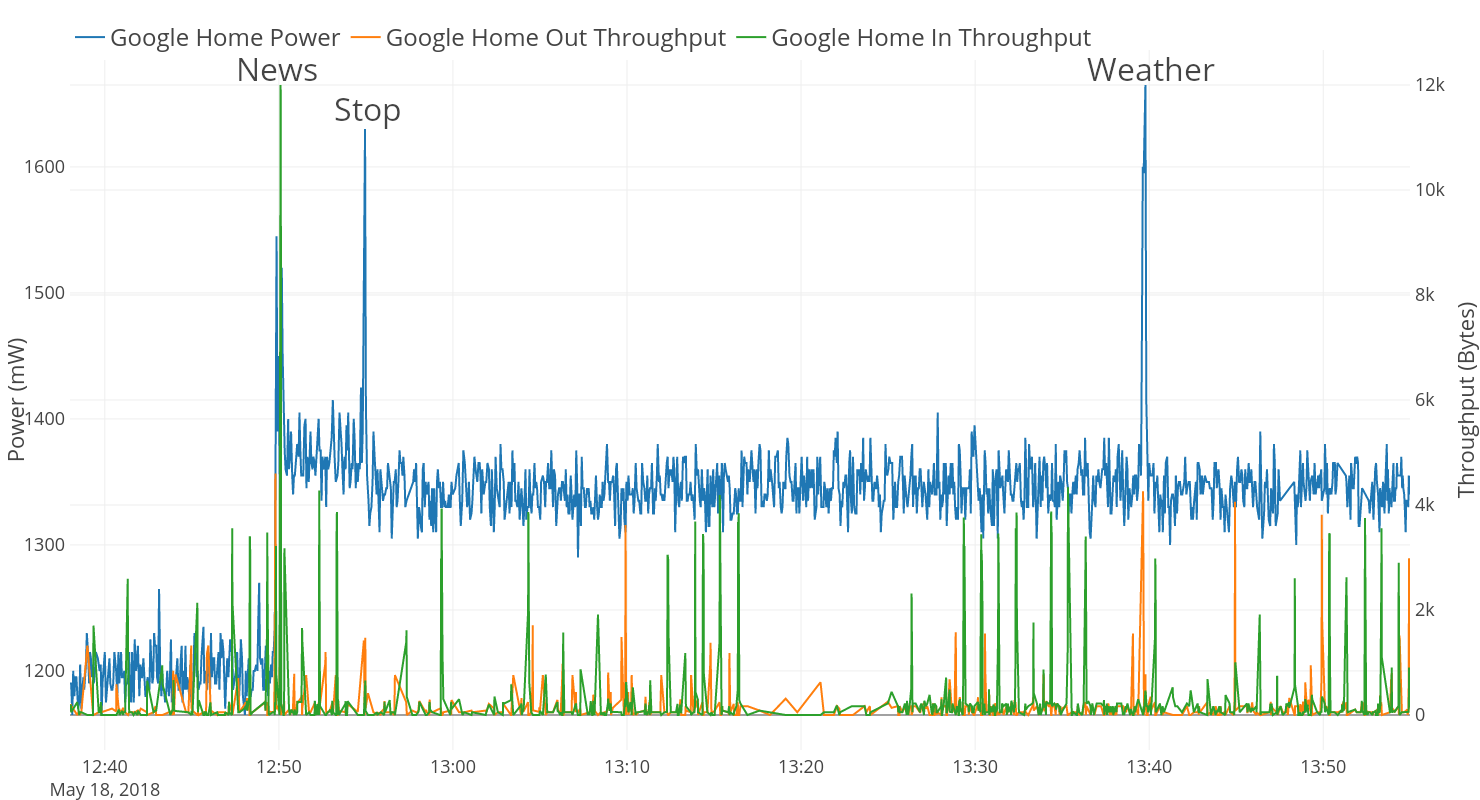
\includegraphics[width=1\textwidth]{homequery}
  \caption{Home Mini Response to News and Weather}
  \label{fig:homequery}
\end{figure}

\subsection{Echo Dot}

One interesting finding from the Echo Dot is that it has a light monitor. When we turn on the lights, the LEDs on the Echo Dot brightens to adapt. The brightness change causes the Echo Dot to use more idle power as shown in figure \ref{fig:echolights}.

\begin{figure}[H]
  \centering
    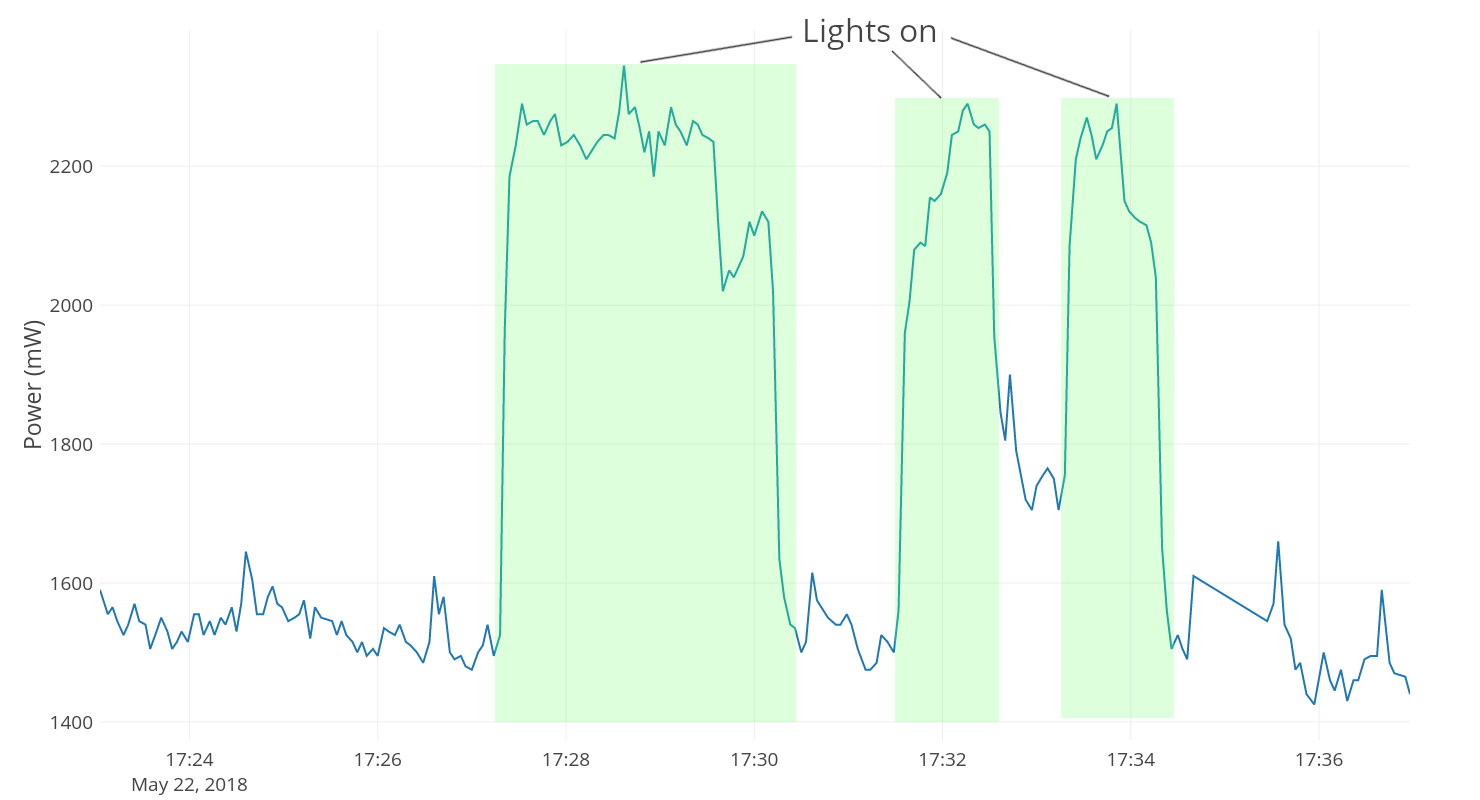
\includegraphics[width=1\textwidth]{echolights}
  \caption{Echo Dot Response to Lights}
  \label{fig:echolights}
\end{figure}

\section{Streaming Devices}
\label{Streaming Devices}

Each subsection shows the streaming devices usage during startup and when streaming.

\subsection{Google Chrome Cast}
\begin{figure}[H]
  \centering
  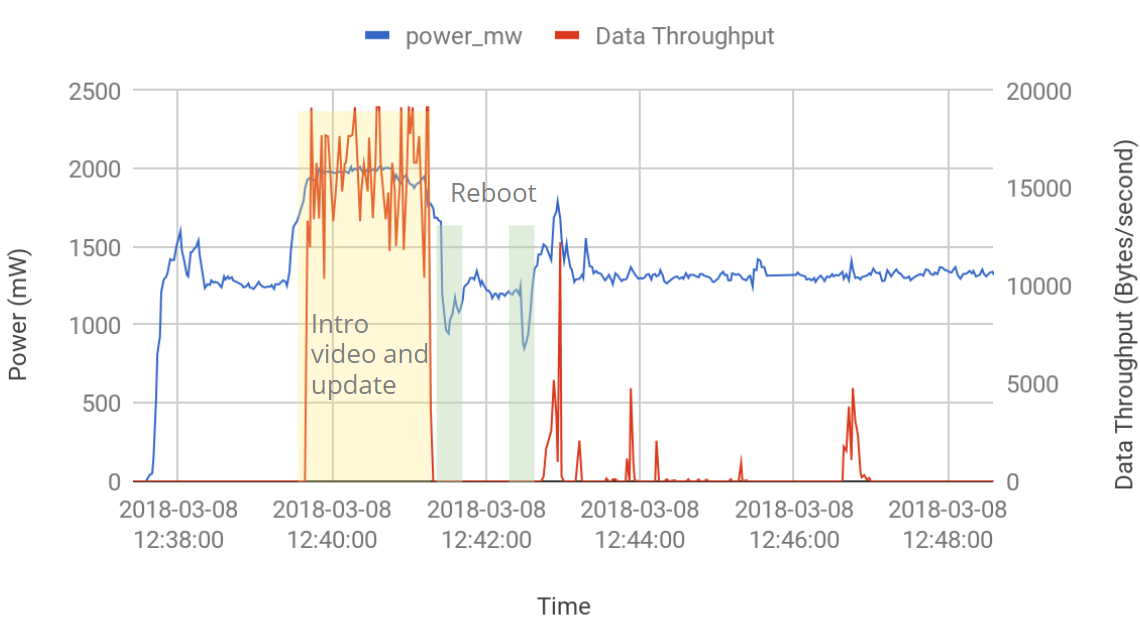
\includegraphics[width=1\textwidth]{ccboth}
  \caption{Chromecast First Time Boot Network Traffic and Power Consumption}
  \label{fig:ccboth}
\end{figure}

The Chrome Cast startup graph is shown in figure \ref{fig:ccboth}. On startup, the Chrome Cast shows an intro tutorial video and downloads a firmware update. After rebooting twice, it is ready to go.

\begin{figure}[H]
  \centering
  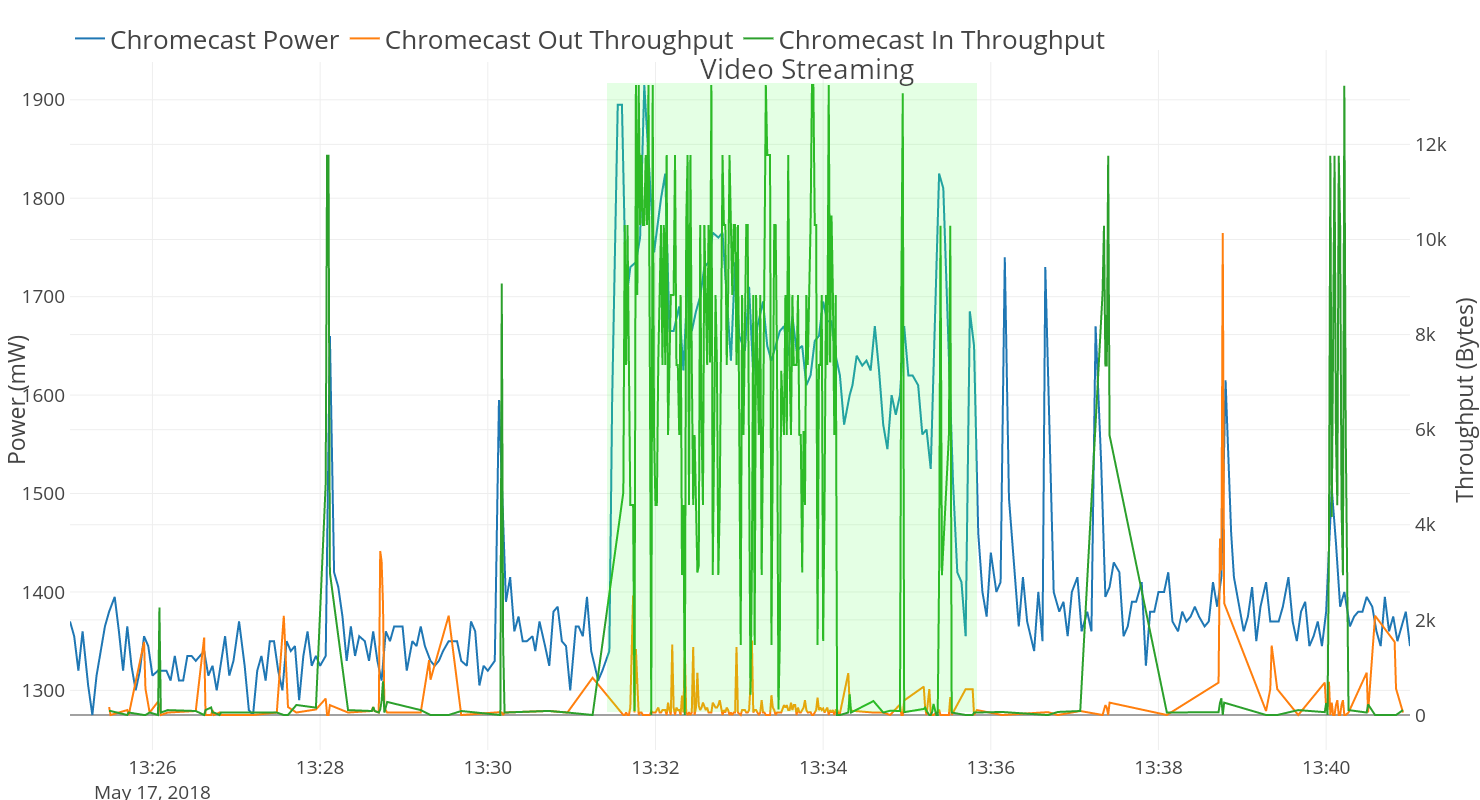
\includegraphics[width=1\textwidth]{ccstreaming}
  \caption{Chromecast Video Streaming}
  \label{fig:ccstream}
\end{figure}

The Chrome Cast streaming graph is shown in figure \ref{fig:ccstream}. In this time frame, the chrome cast streams video in the marked box.

\begin{figure}[H]
  \centering
  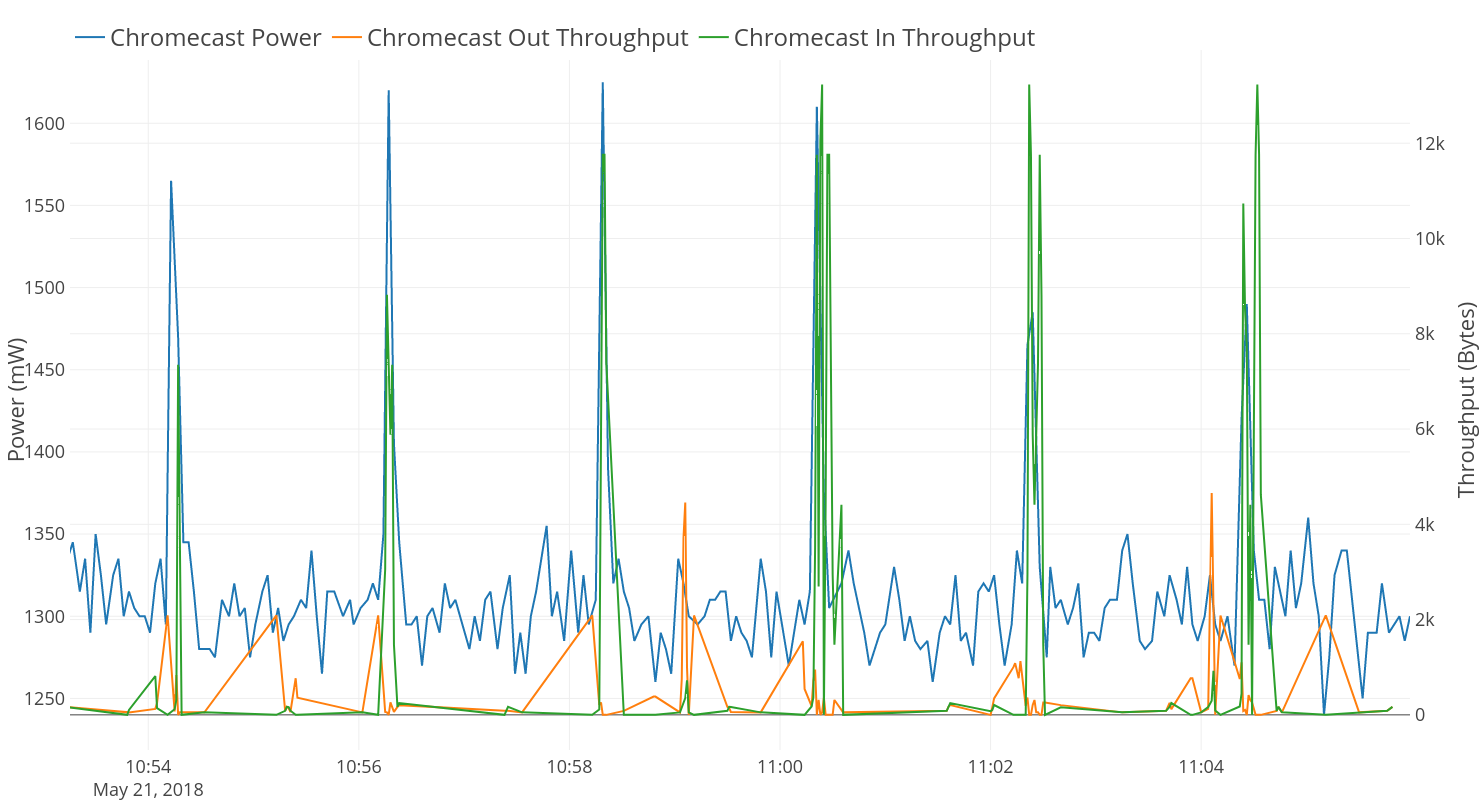
\includegraphics[width=1\textwidth]{chromecastbg}
  \caption{Chromecast Idle Traffic}
  \label{fig:ccbg}
\end{figure}

Additionally, the Chrome Cast idle graph is shown in figure \ref{fig:ccbg}. In this time frame, there are consistent spikes to the chrome cast every 2 minutes. During these spikes, the chrome cast is showing a new background that it downloads from Google Servers.

\subsection{Amazon Fire Stick}

\begin{figure}[H]
  \centering
  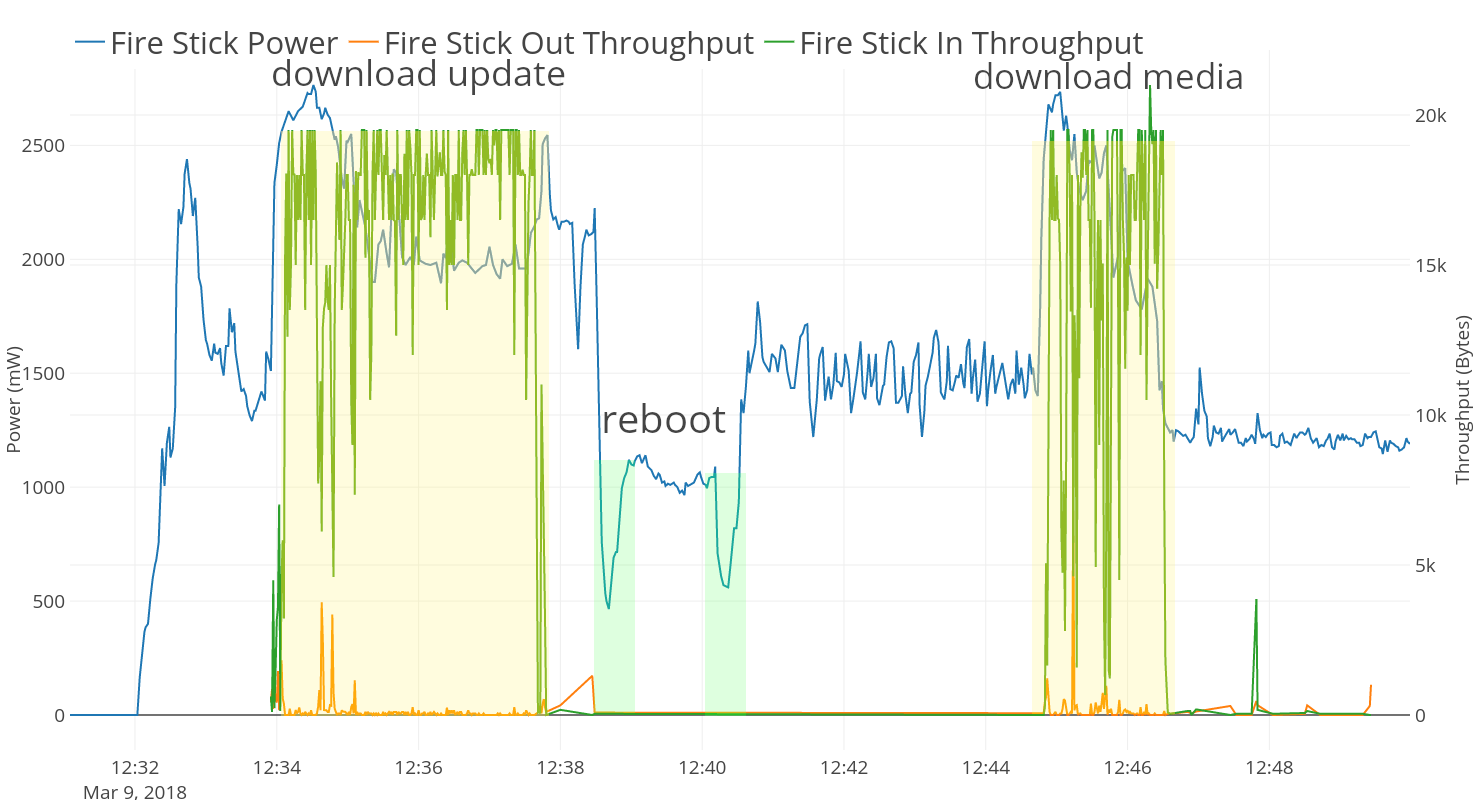
\includegraphics[width=1\textwidth]{fireboot}
  \caption{Fire TV Stick First Time Boot Network Traffic and Power Consumption}
  \label{fig:fireboth}
\end{figure}

The Amazon Fire Stick startup graph is shown in figure \ref{fig:fireboth}. On first boot, the fire stick downloads an update, reboots twice, then downloads certificates from Symantec and Verisign.

When streaming, the Fire Stick increases throughput and power usage with a spike at the beginning and end of streaming in power usage as shown in figure \ref{fig:fsyt}.

\begin{figure}[H]
  \centering
  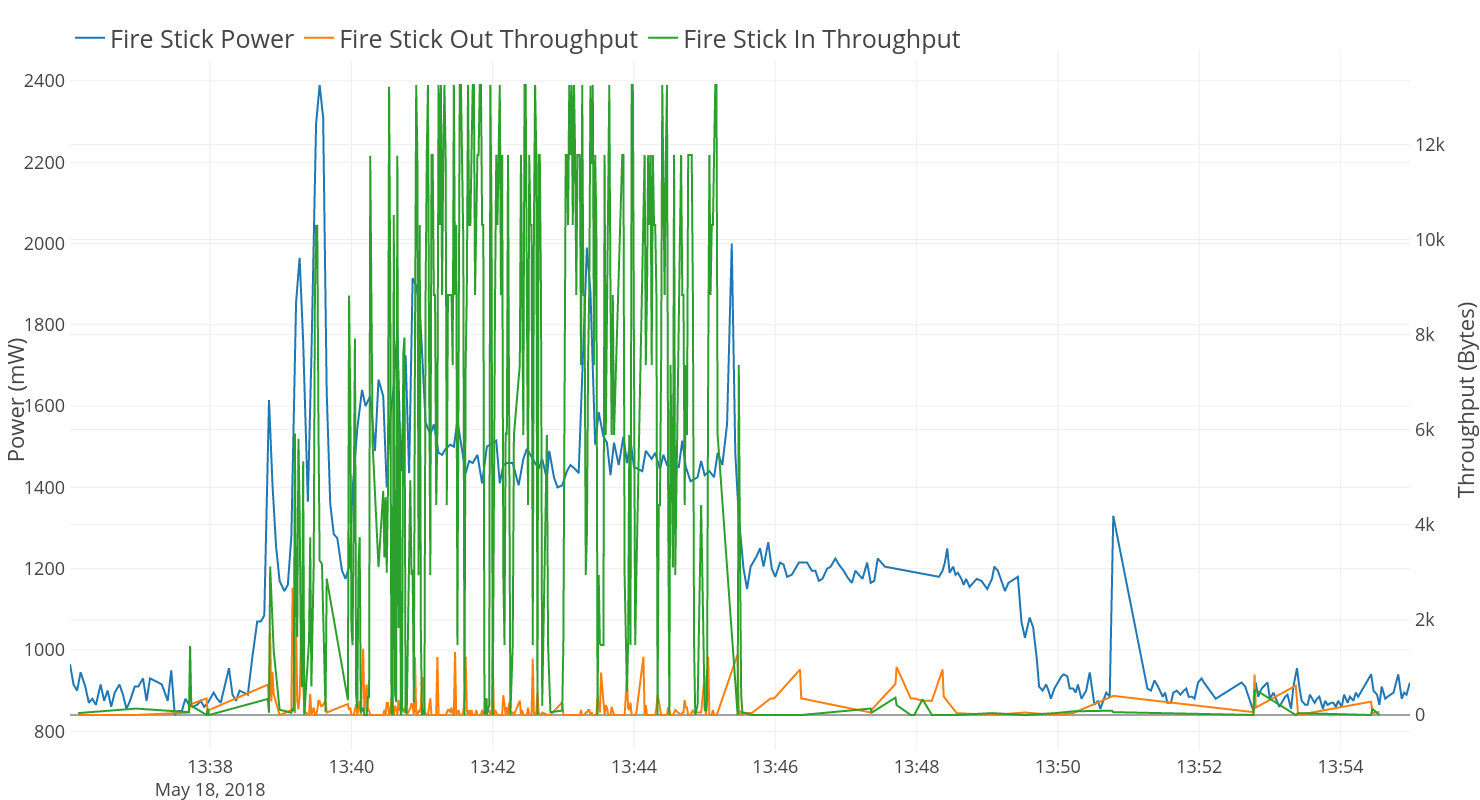
\includegraphics[width=1\textwidth]{fsyt}
  \caption{Fire TV Stick Video Streaming}
  \label{fig:fsyt}
\end{figure}

\subsection{Roku Express}
When streaming, the Roku's power usage and network throughput rise and stay at a constant level until the video streaming is complete. At which point it drops back down when done.

\begin{figure}[H]
  \centering
  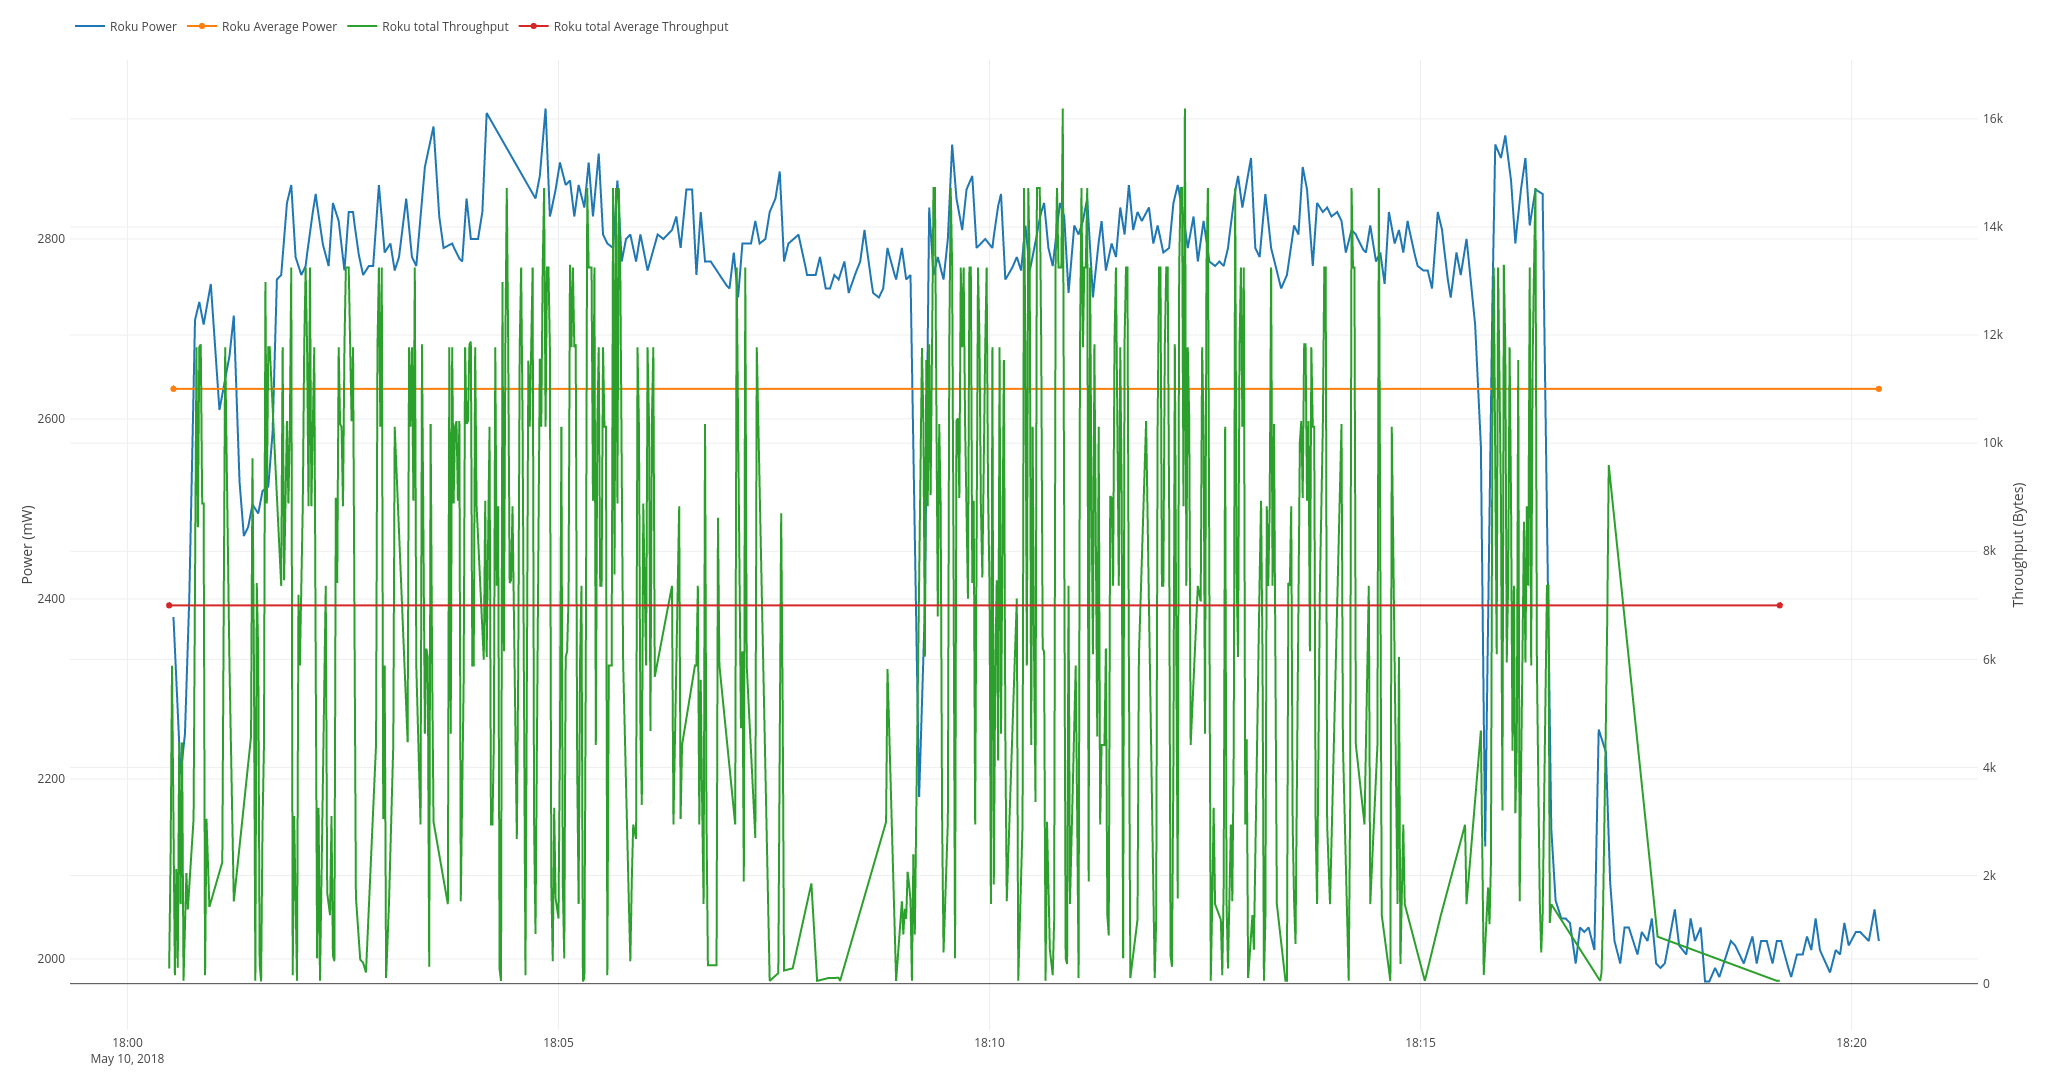
\includegraphics[width=1\textwidth]{figures/rokuStreaming.png}
  \caption{Roku Express Video Streaming}
  \label{fig:rokuStreaming}
\end{figure}

\section{Summed Power Graph}
\label{sumPowerGraph}
In this section, we show graphs of the five smart speakers summed up as one graph of power usage. The devices used includes two echo dots, 2 Eufy genies, and 1 Google chrome cast.

\begin{figure}[H]
  \centering
  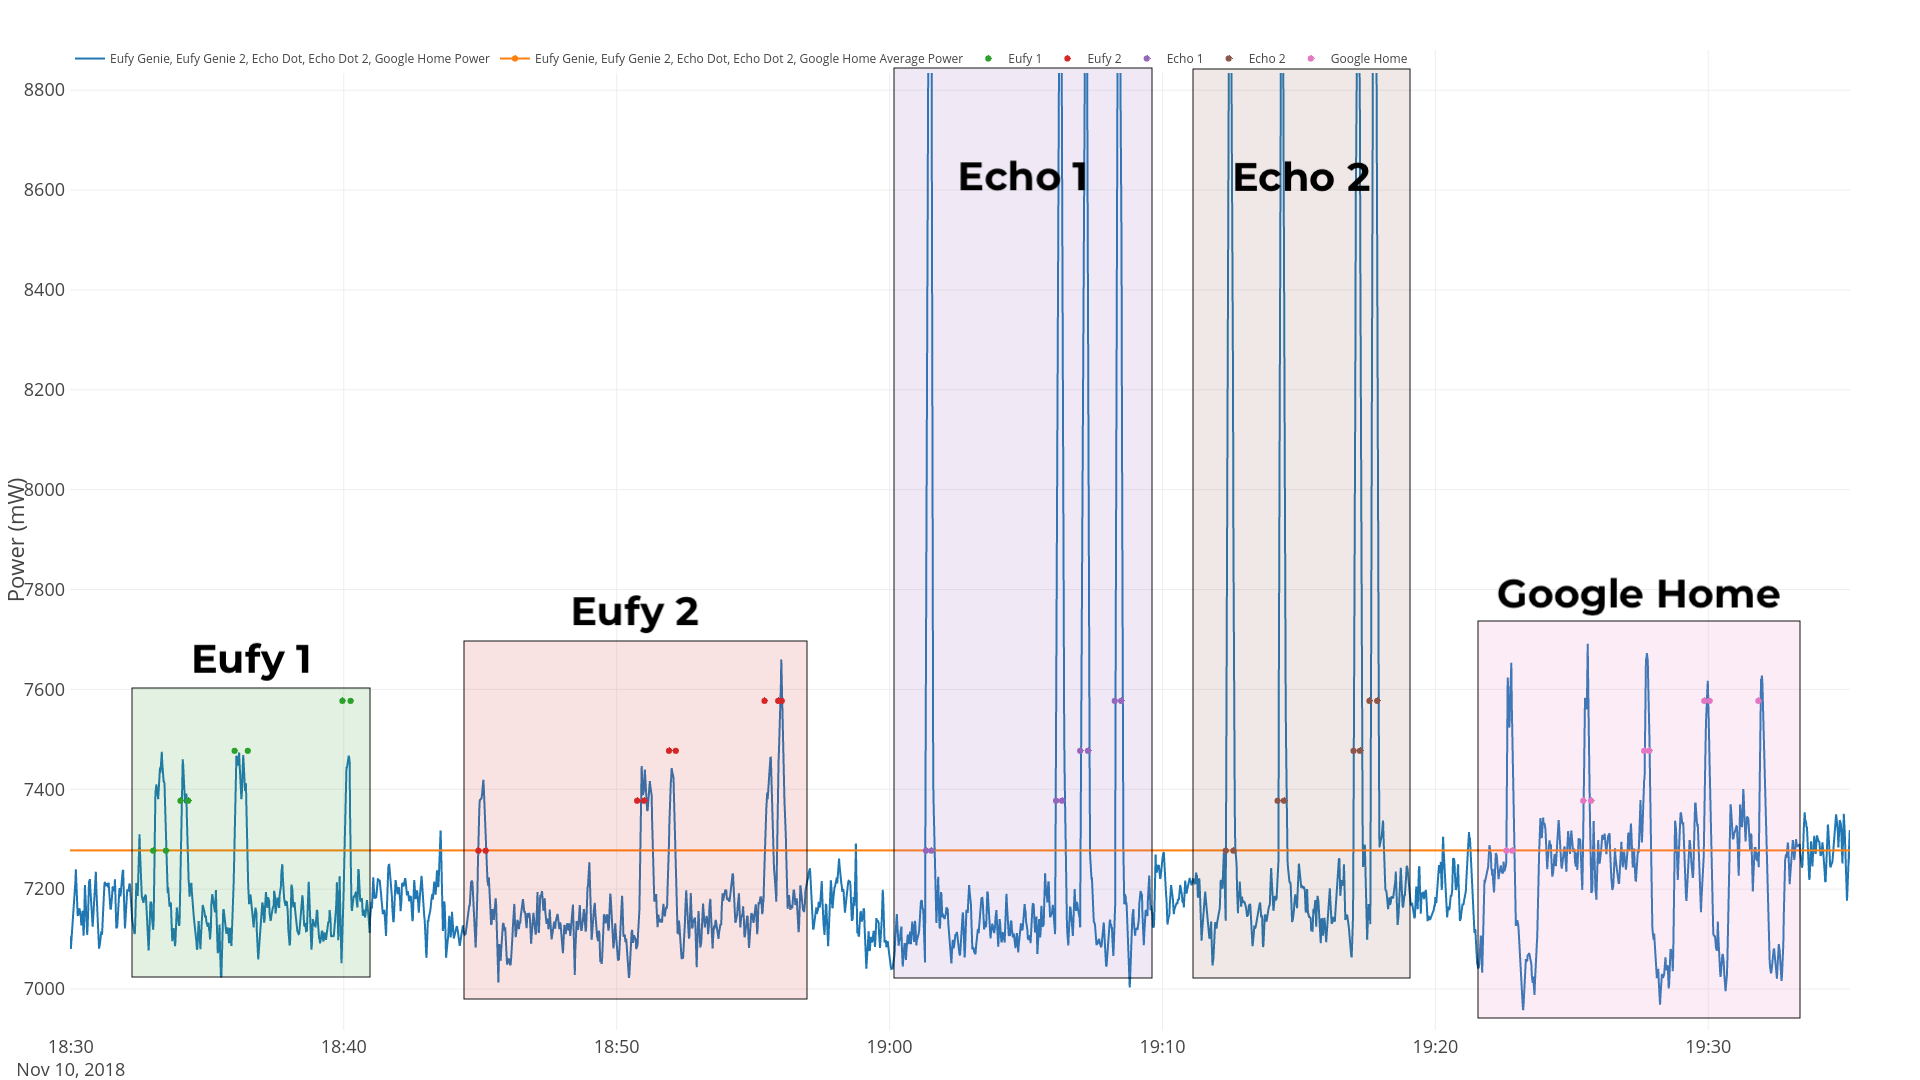
\includegraphics[width=1\textwidth]{figures/weatherSum.png}
  \caption{5 Smart Speakers Power Summed Up. Toggled the mute button and queried each device for the weather.}
  \label{fig:weatherSum}
\end{figure}

The first graph \ref{fig:weatherSum} is shown in a time frame where each device is unmuted and muted for a period. We wanted to see if muting and unmuting the devices changed anything. In this graph, there are changes, but they do not correlate to the muting/unmuting. We did this a few more times and found that most of the time, the power usage stayed the same. Then we queried each smart speaker for the weather while all other smart speakers were muted at the 18:30 mark. We queried each device in order 3-4 times in consecutive order so that it is easy to see and to check for consistent results. The Eufy had the smallest spike for this command at 400 mW, then the google home at 600 mW, and finally the echo dot at 2000 mW.

\begin{figure}[H]
  \centering
  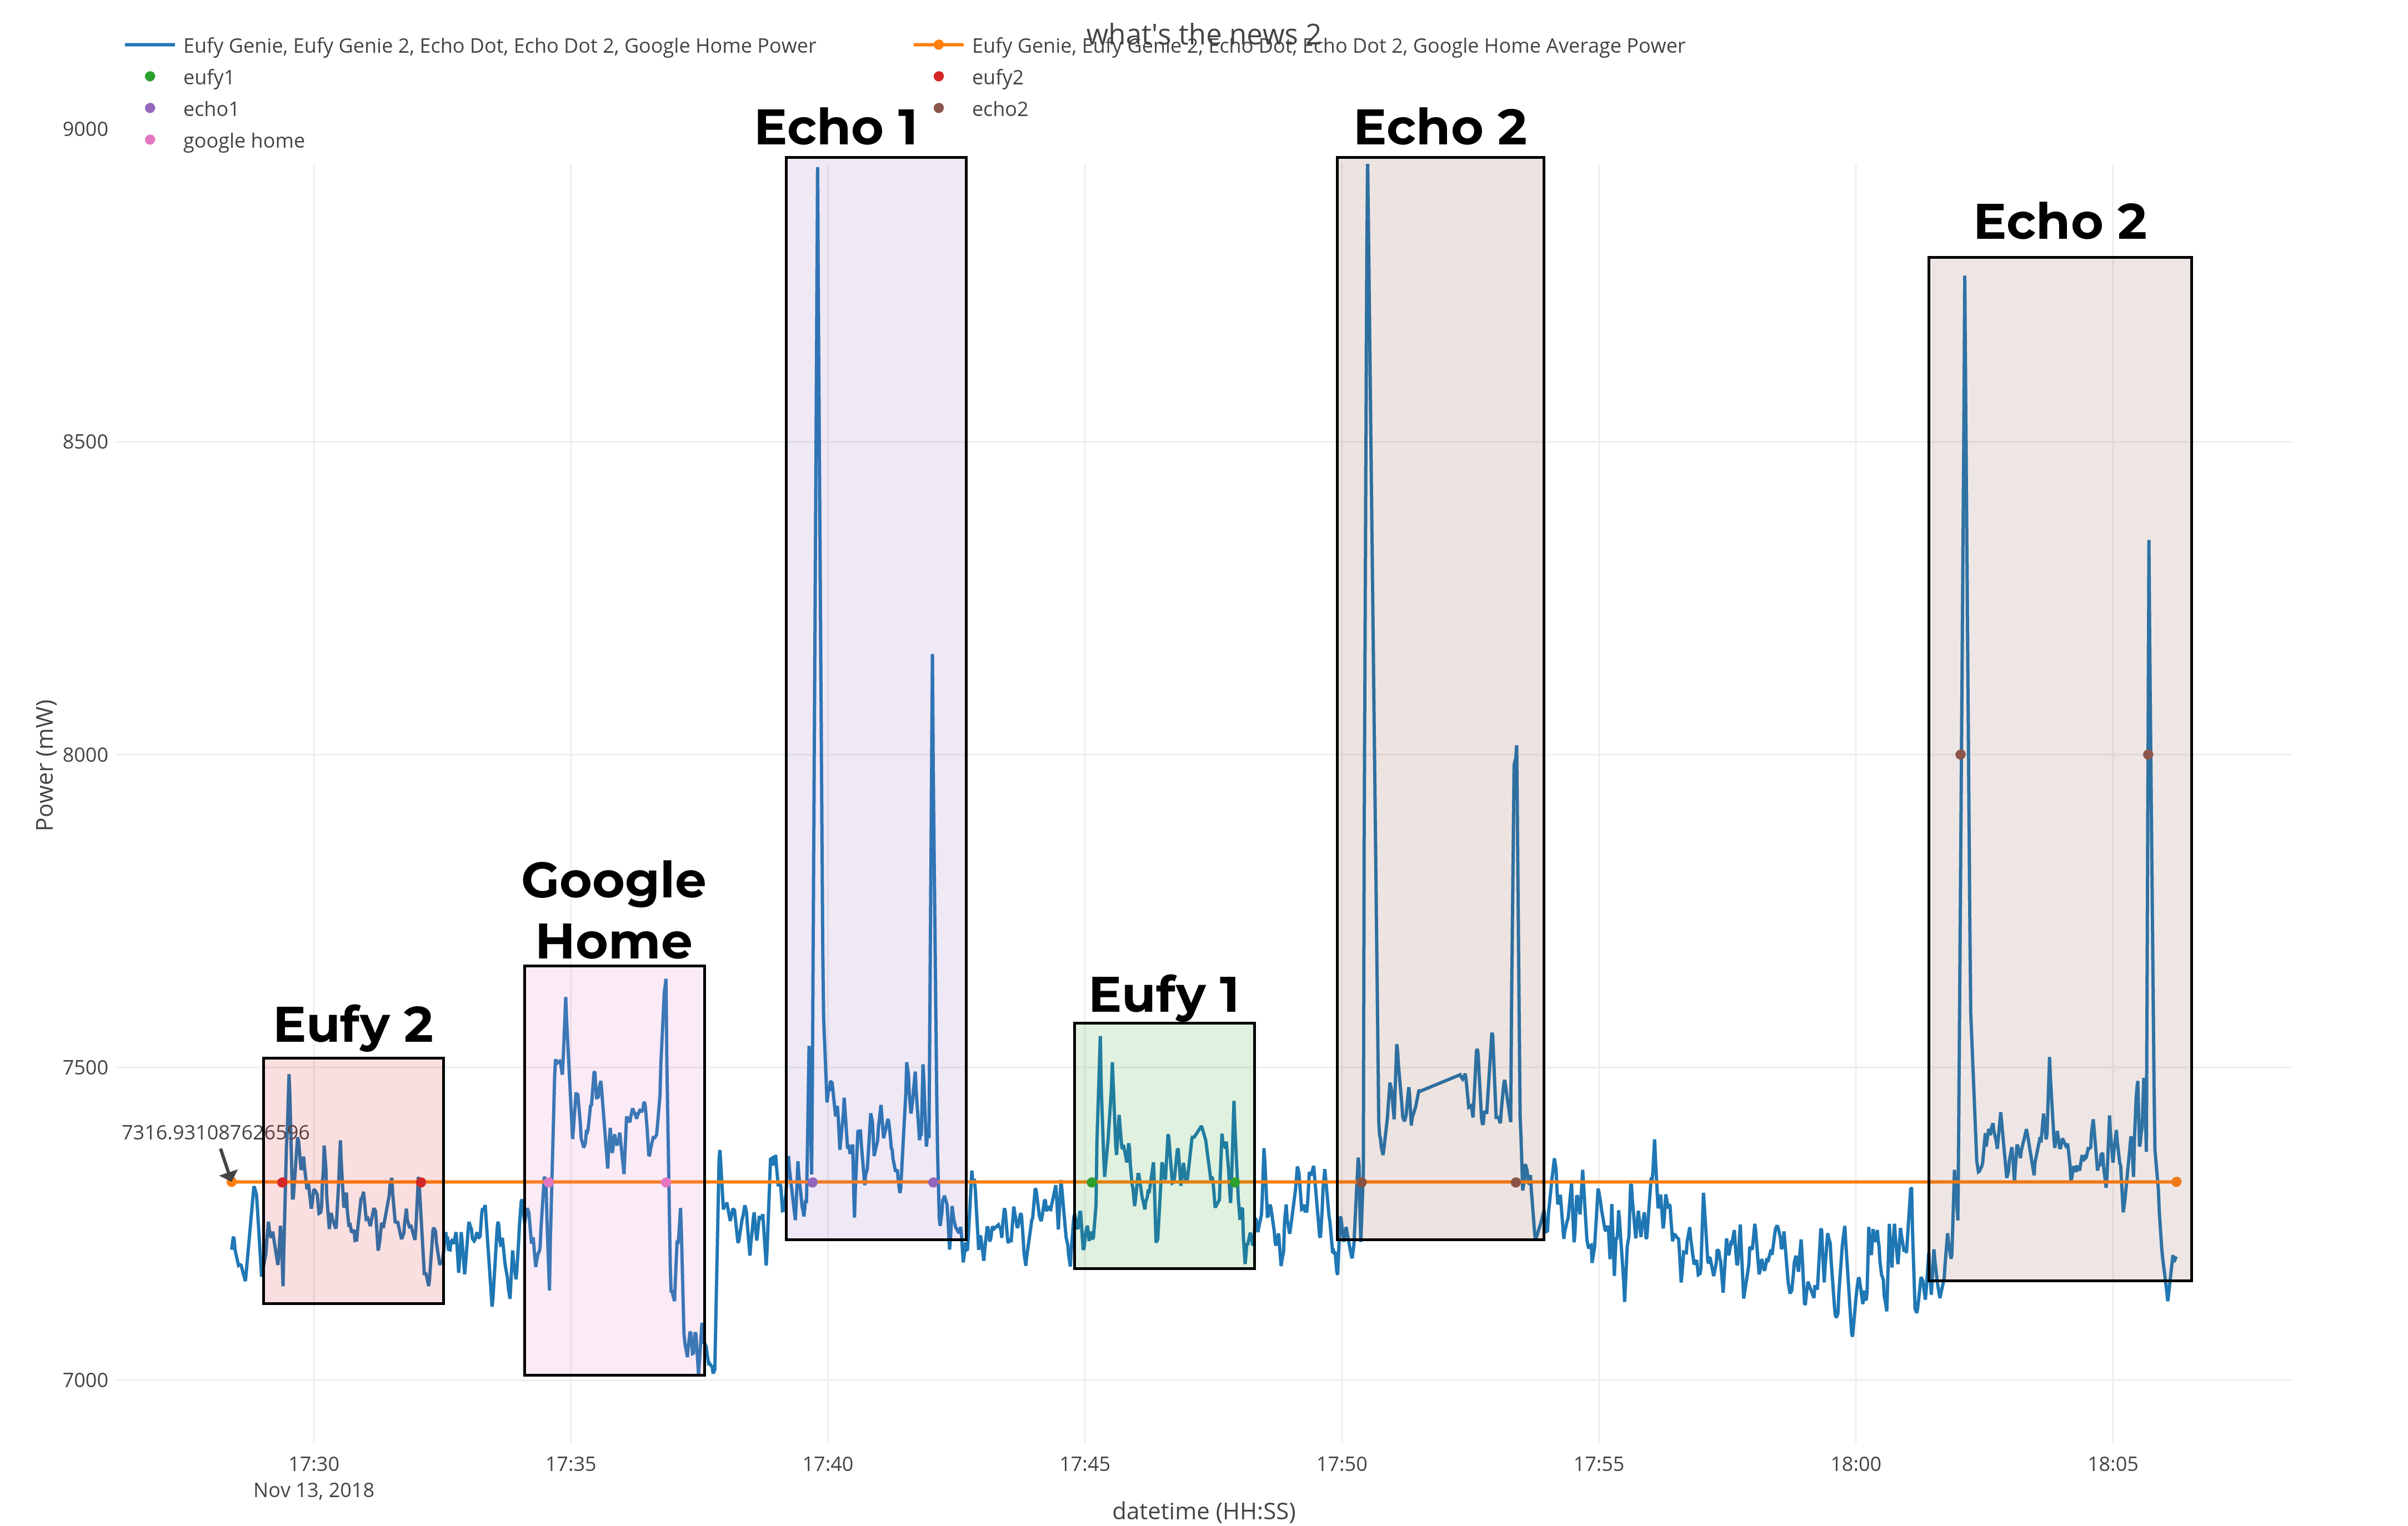
\includegraphics[width=1\textwidth]{figures/mixedNewsSum.png}
  \caption{5 Smart Speakers Power Summed Up. Queried each device for the
  news.}
  \label{fig:mixedNewsSum}
\end{figure}

The next graph \ref{fig:mixedNewsSum} shows the smart speakers when asked for the news. We asked each device for the news at random as to prevent any optimizations. This graph and the rest of the summed graphs in this section use the same notation for signifying commands. Two corresponding dots of the same color signify the start and end of the command for a specific device. If the dots are on another level, then this command has been repeated another time.

In this graph, all devices have a spike at the beginning and end of the command and maintain a steady energy usage in between that is slightly higher than the idle energy used. The peak to peak spike of the Eufy Genie is the smallest at 350 mW, then the Google Home at 500 mW, and finally the Echo Dot at 1900 mW.

\begin{figure}[H]
  \centering
  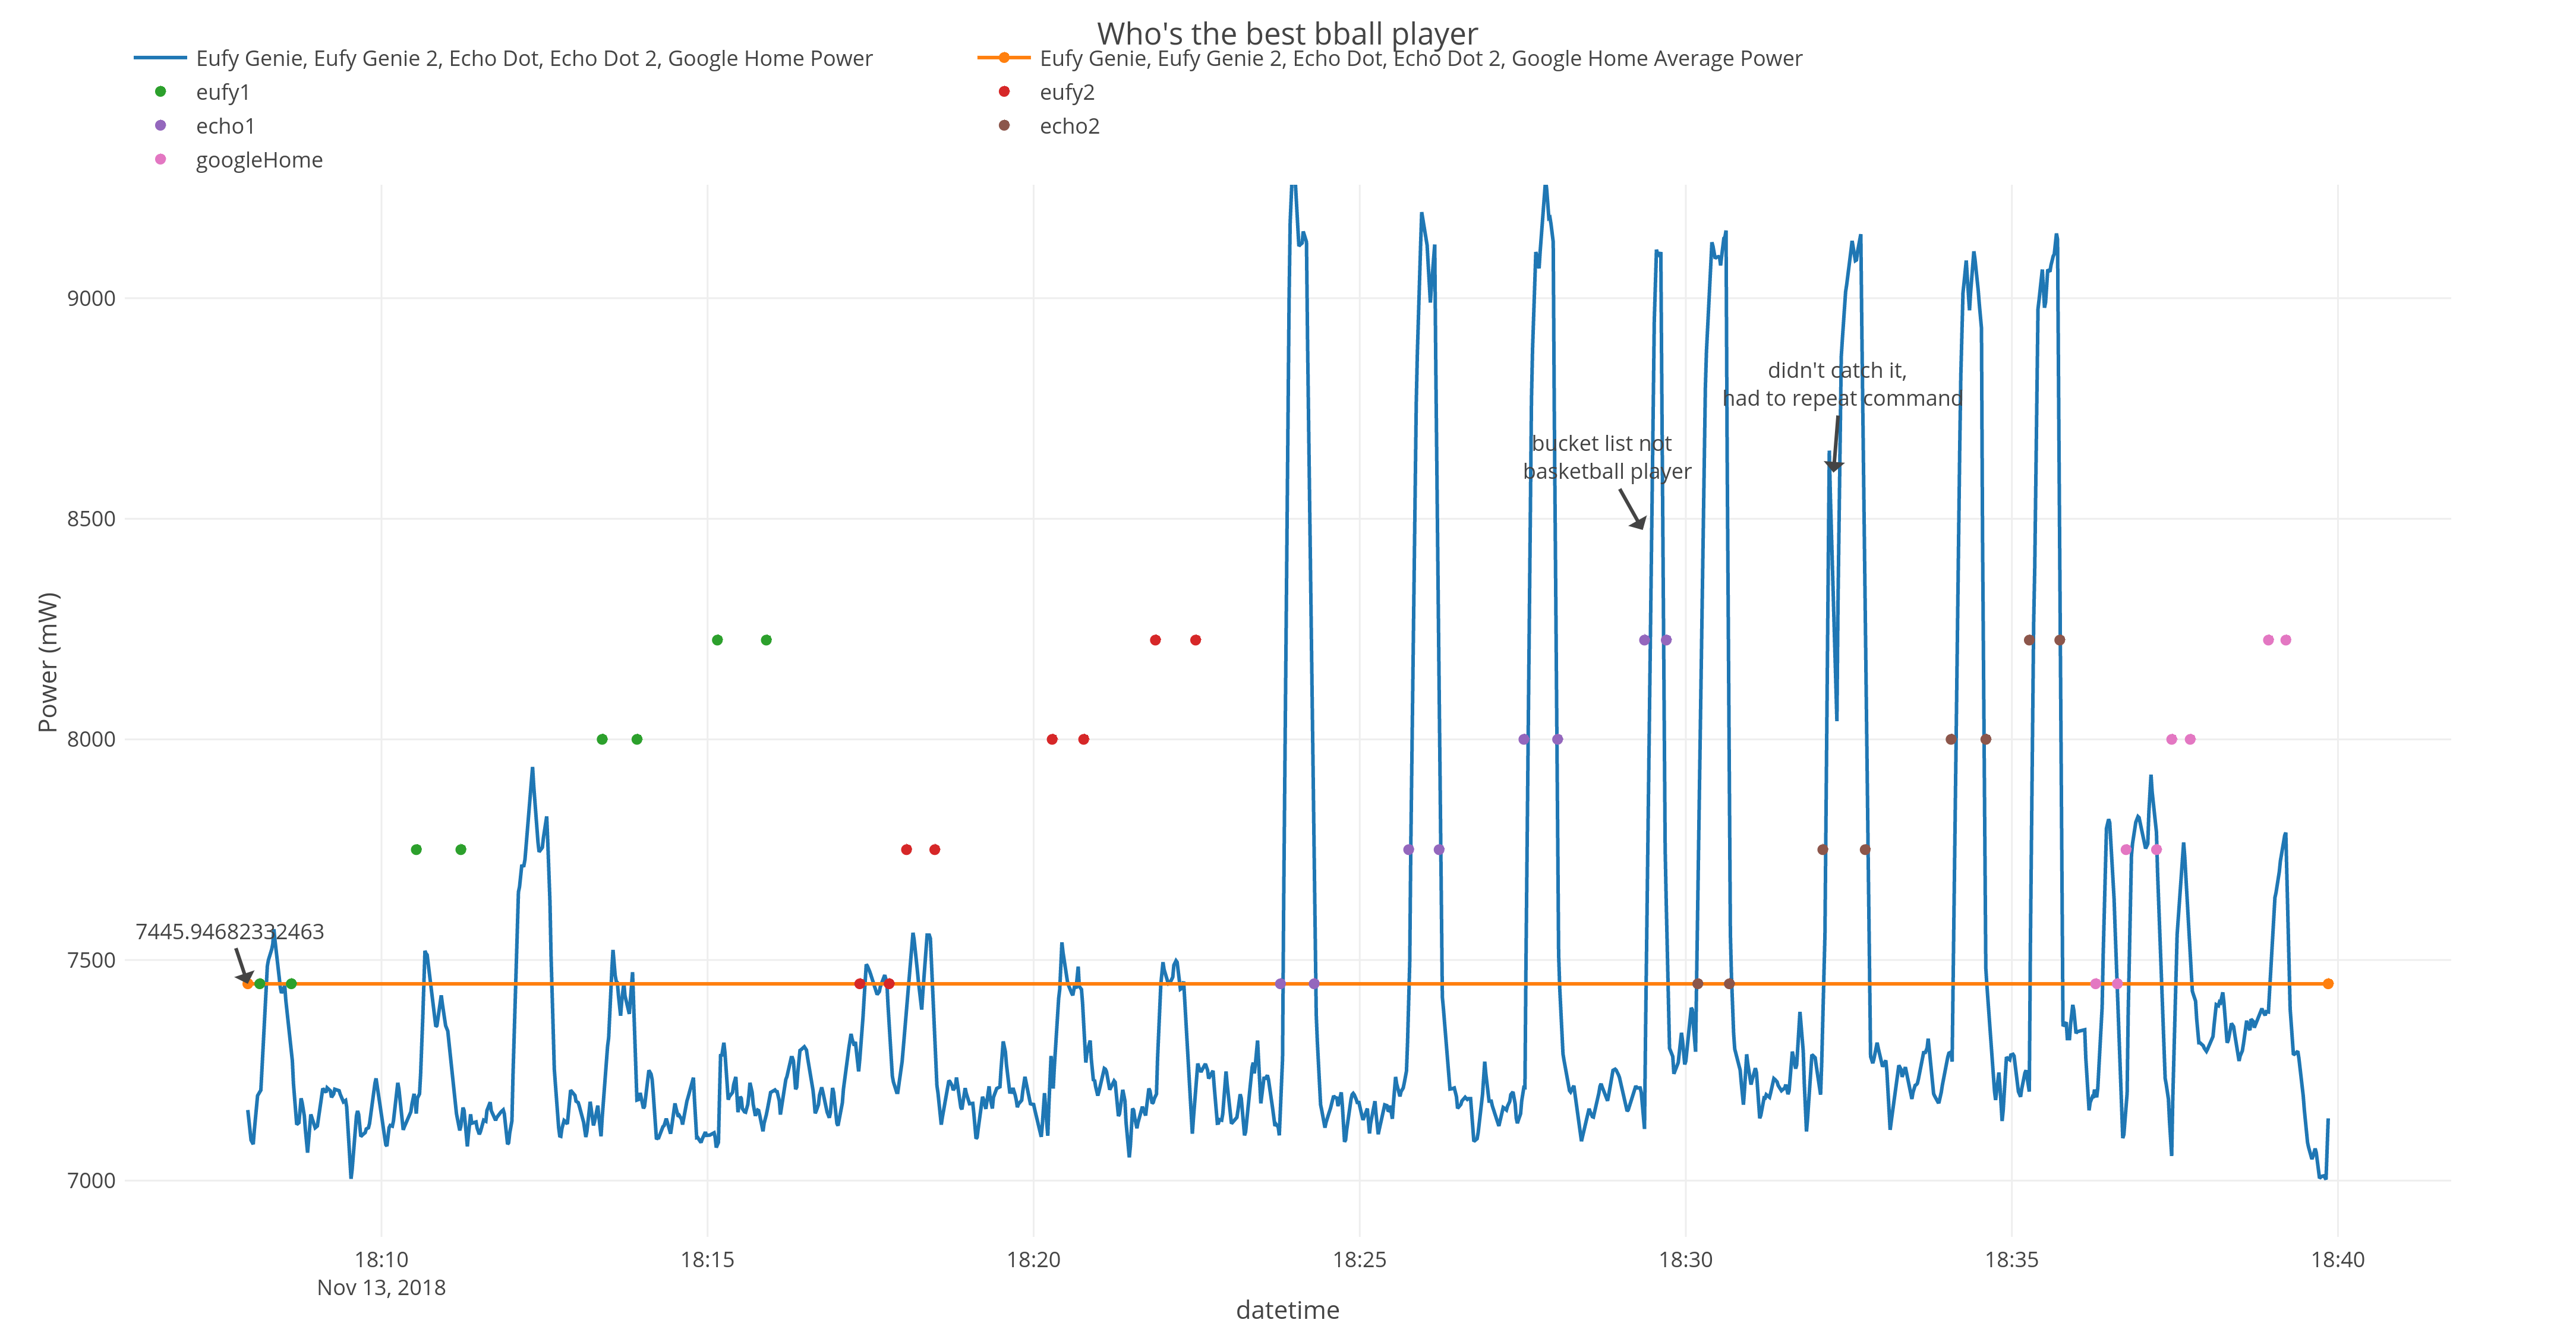
\includegraphics[width=1\textwidth]{figures/bestBballSum.png}
  \caption{5 Smart Speakers Power Summed Up. Queried each device for the
  best basketball player.}
  \label{fig:bestBballSum}
\end{figure}

The next graph \ref{fig:bestBballSum} shows the smart speakers when asked for the best basketball player. The annotation scheme is the same as before. Each smart speaker is queried for the best basketball player in consecutive order four times. Similar to before, the Eufy has a power spike of 420 mW peak to peak, the Google Home has a power Spike of 720 mW, and the Echo Dot has a power spike of 2180 mW.

However, when looking at graph \ref{fig:bestBballSum}, there is a power spike that is unaccounted for in correspondence to the event log. We made a query, invoking all other power spikes but we did not do anything for the power spike at 18:12 that is higher than the other Eufy power spikes.

To figure what the power spike at 18:12 is, we separated the graphs into individual power traces as shown in figure \ref{fig:bestBballSeperate}. From the graph, the power spike at 18:12 is attributed to the Echo Dot 2. We then looked at the individual network usage for each of these devices in this time frame as shown in figure \ref{fig:bestBballNetwork}. At 18:12, there is no significant network usage. We had no conclusive evidence to decide what the power spike is accounted to, but section \ref{Discussion} covers some speculated reasons.

\begin{figure}[H]
  \centering
  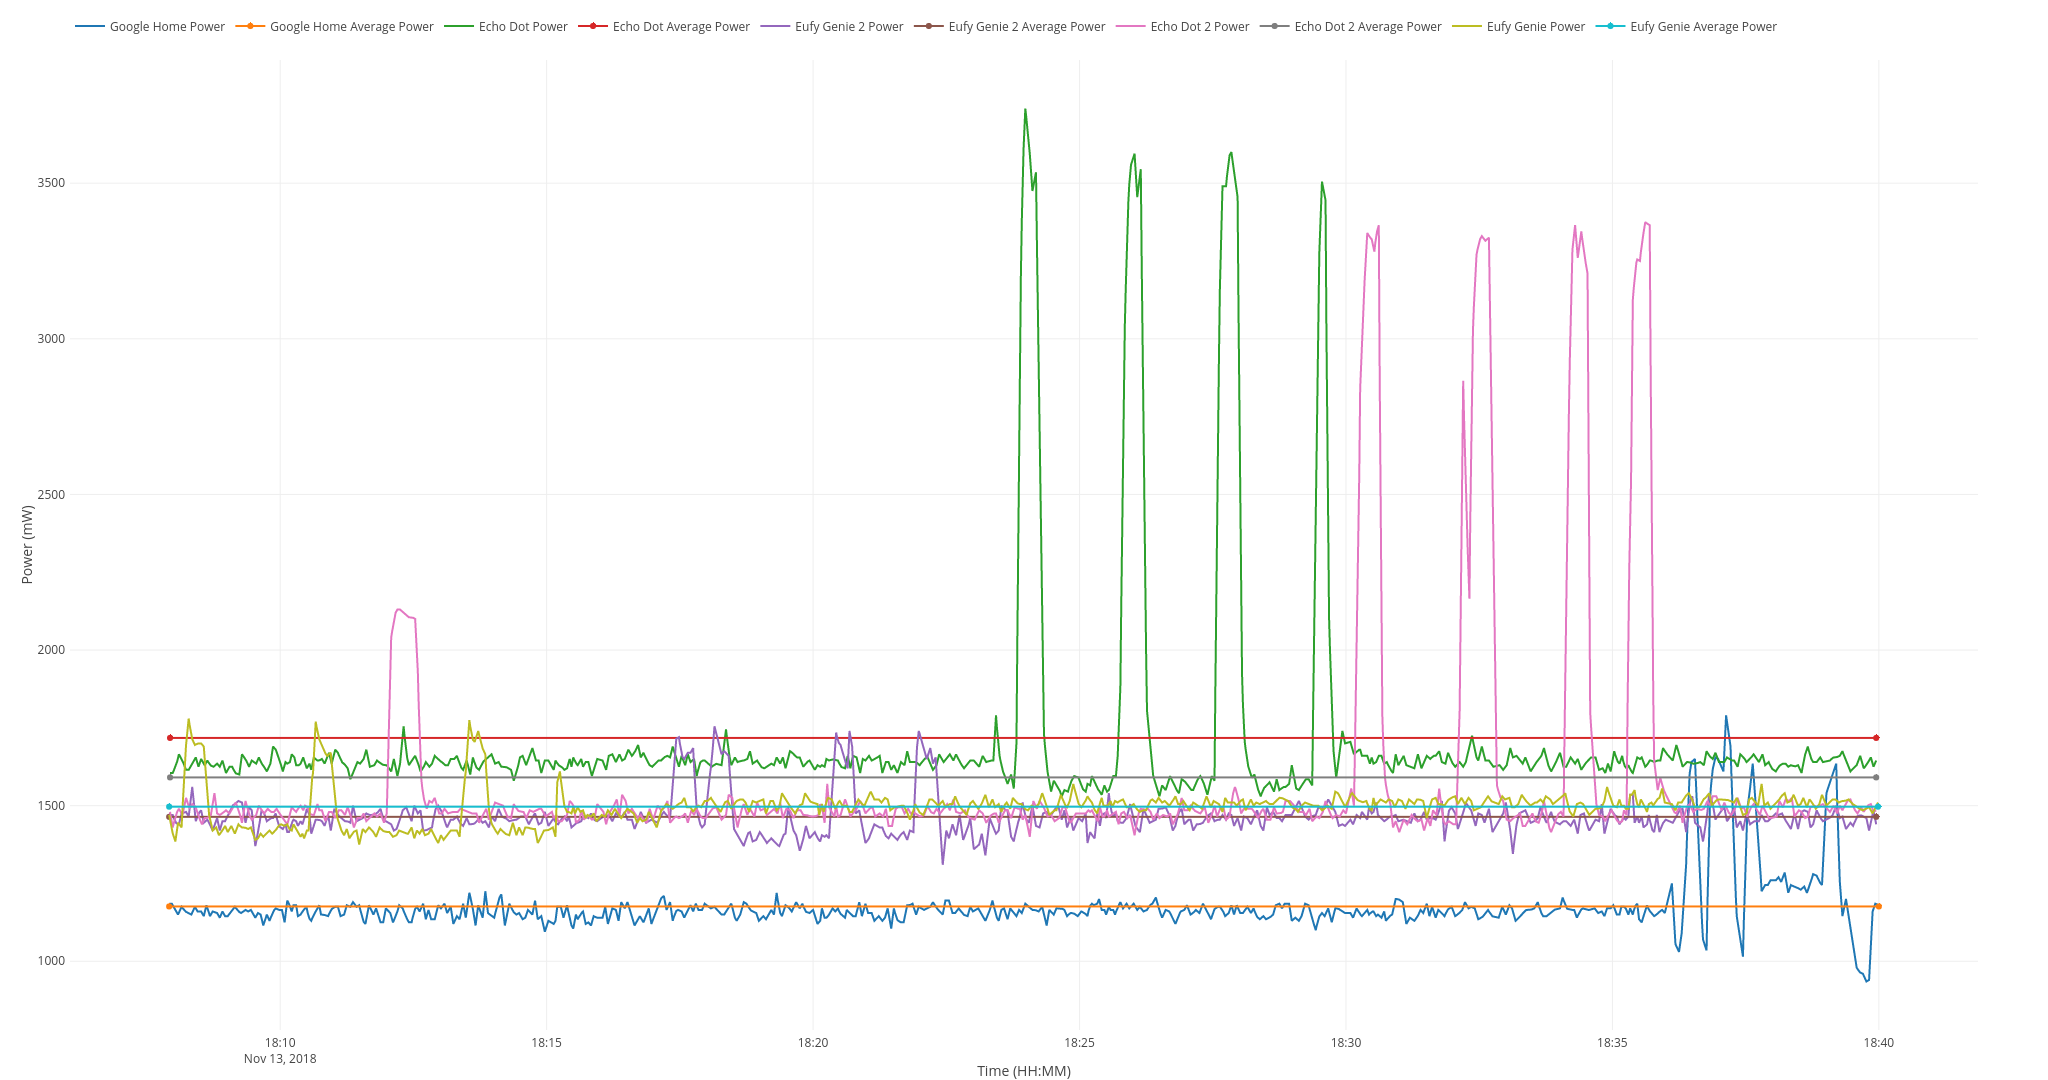
\includegraphics[width=1\textwidth]{figures/bestBballSeperate.png}
  \caption{5 Smart Speakers Power Usage over time. Queried each device for the
  best basketball player.}
  \label{fig:bestBballSeperate}
\end{figure}

\begin{figure}[H]
  \centering
  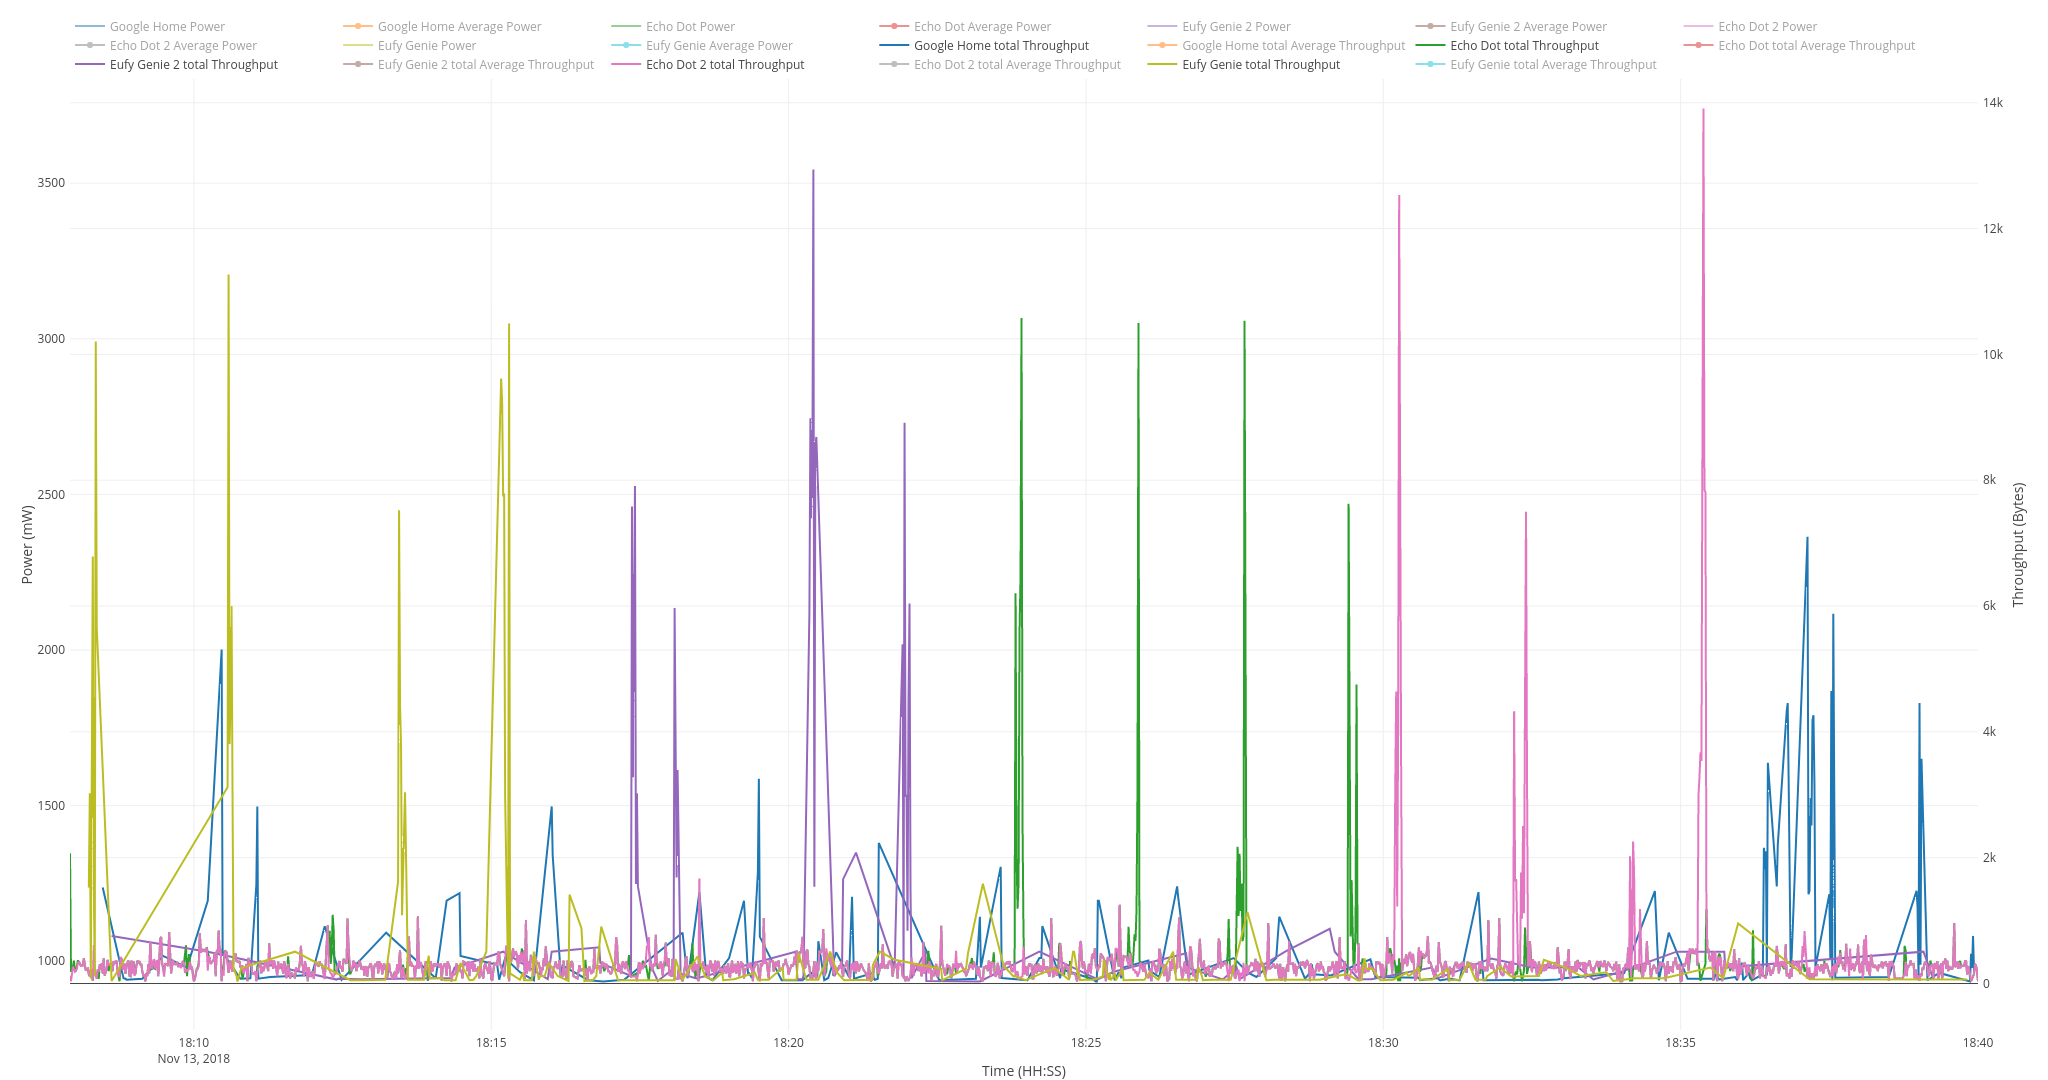
\includegraphics[width=1\textwidth]{figures/bestBballNetwork.png}
  \caption{5 Smart Speakers Network throughput over time. Queried each device for the best basketball player.}
  \label{fig:bestBballNetwork}
\end{figure}

The power spike information for each query type (``what's the weather'' ``what's the news'', ``who's the best basketball player'') are shown below in figure \ref{fig:spikeVoltages}. This bar graph also includes the average spike height for each device over these three commands. The black line at the top of each bar shows the standard deviation. Averaging peak to peak voltage spikes for each device shows the Eufy Genie with a 390 mW spike with 36.1 mW standard deviation, the Google Home with a 606.7 mW spike with 110 mW standard deviation, the Echo Dot with a 2026.7 mW spike with 149.89 mW standard deviation.

\begin{figure}[H]
  \centering
  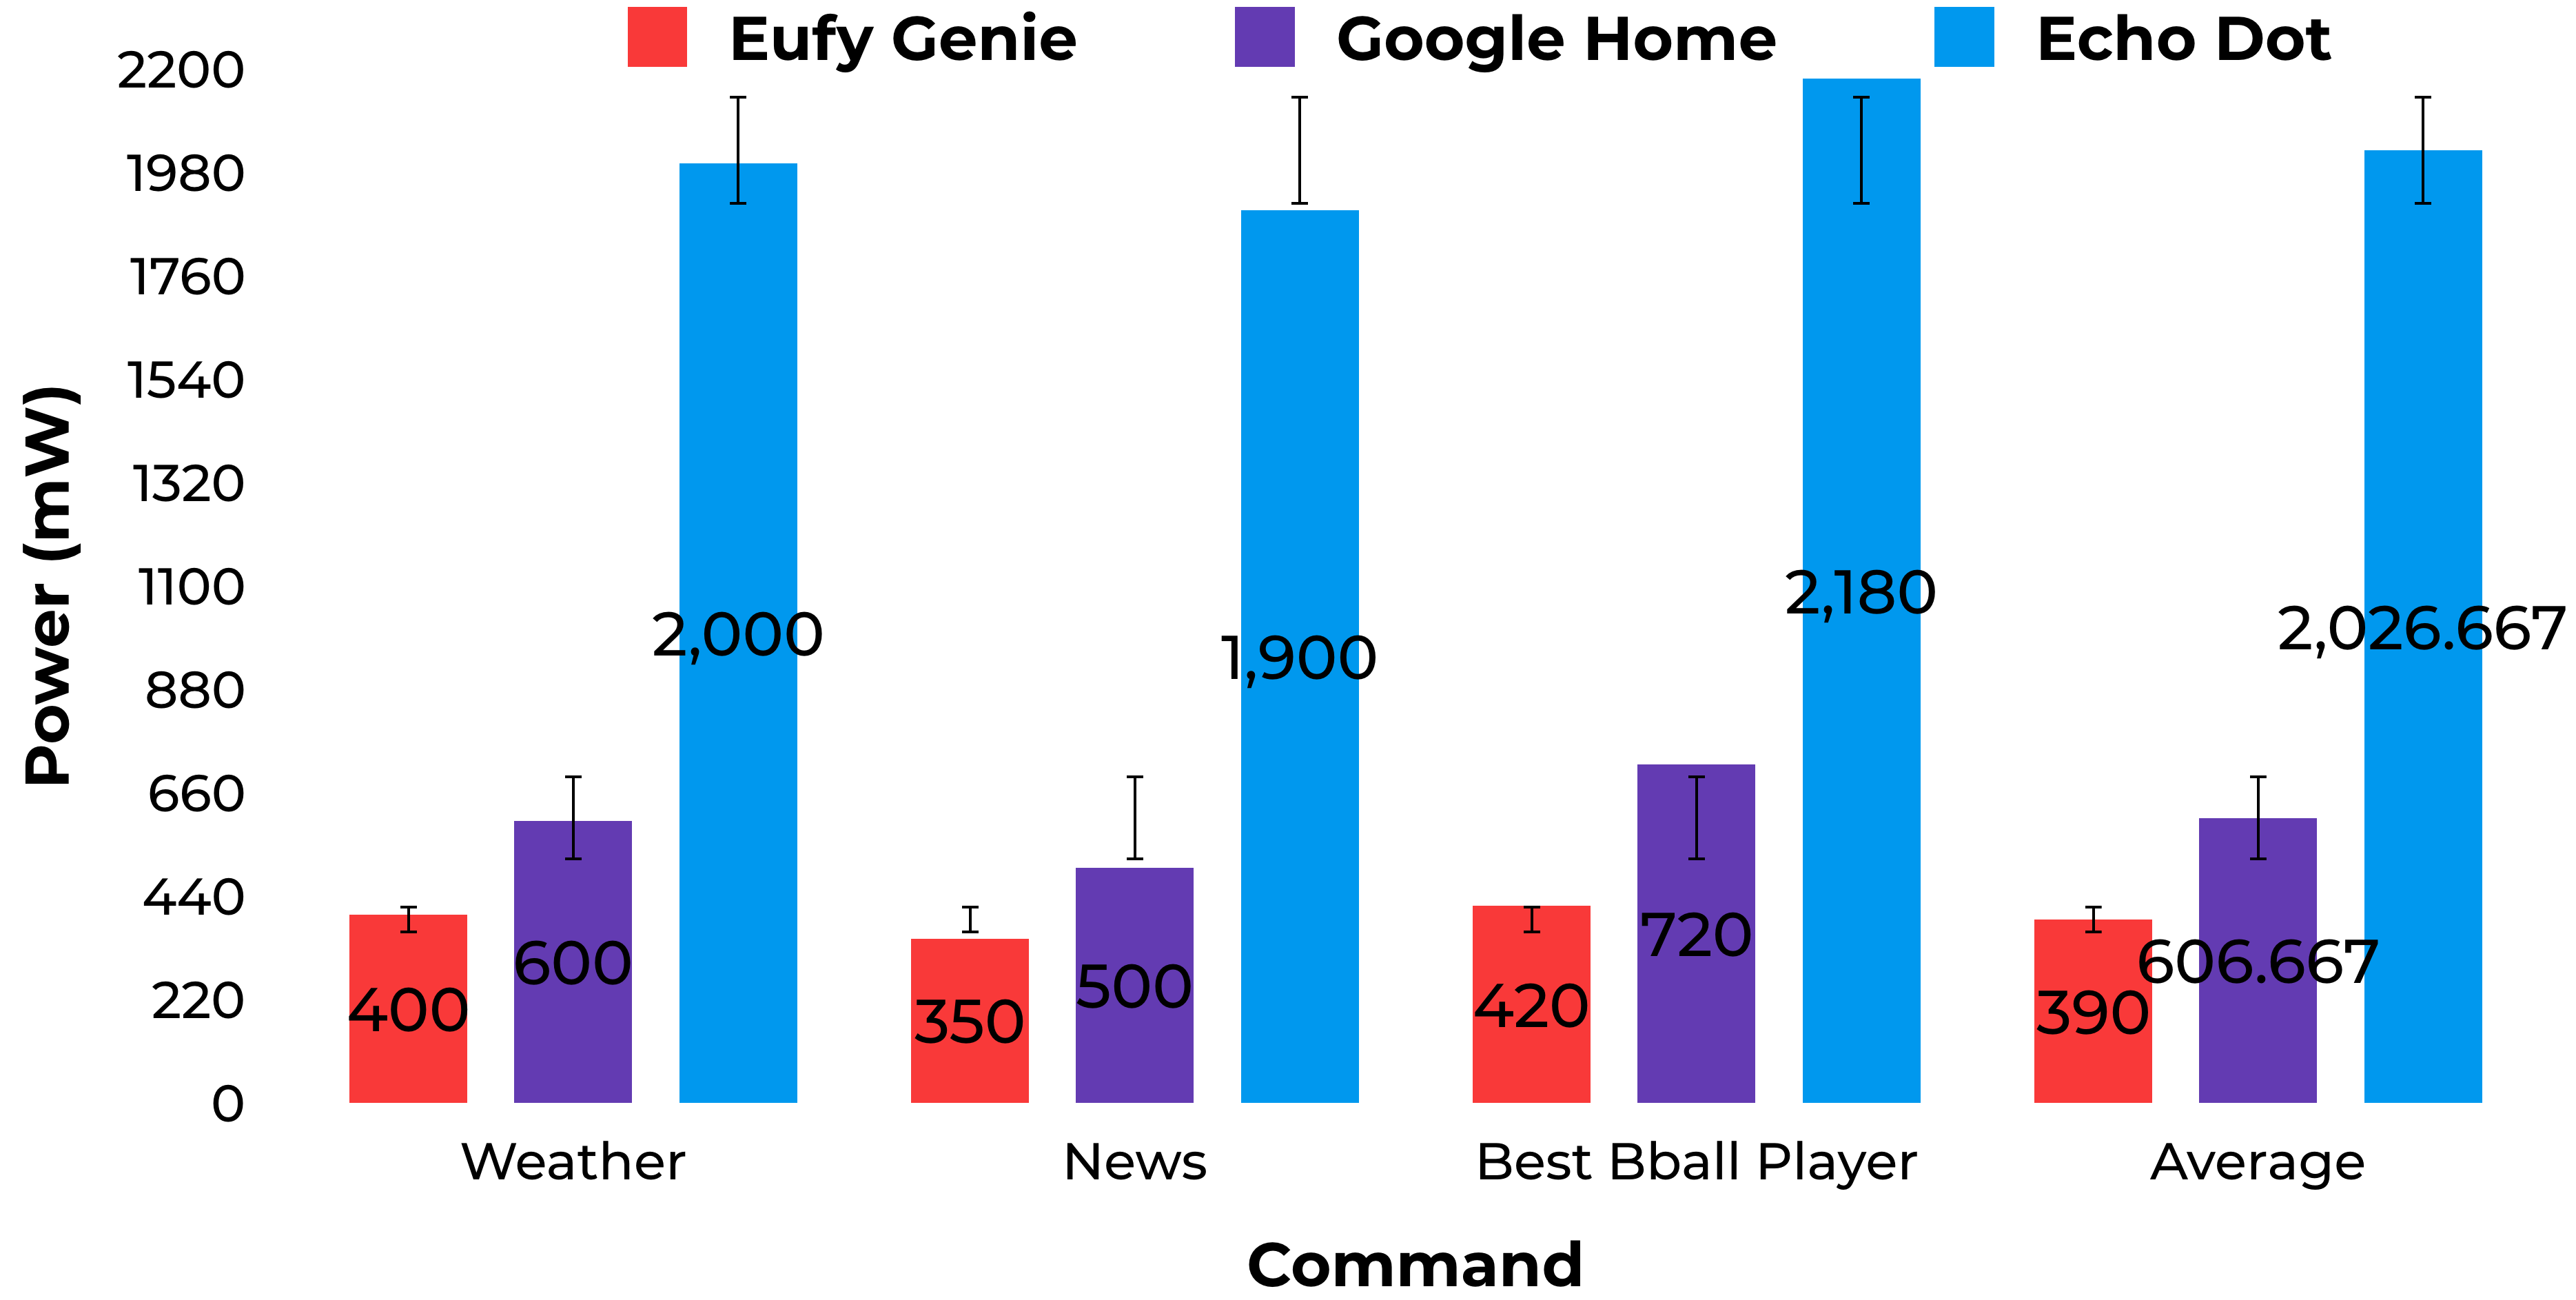
\includegraphics[width=1\textwidth]{figures/spikeVoltages.png}
  \caption{Spike summary of for each query.}
  \label{fig:spikeVoltages}
\end{figure}

\section{Summed Power Graph With Noise}
\label{sumPowerGraphWithNoise}
In this section, we introduce noise into the system so that we can determine if the power spike from each smart speaker is still discernible within a summed power graph when we add high power devices.

In each subsection, there are three traces. The first trace (blue trace) is the power usage over time for a high power device. This trace maps to various devices as we switch them out. The second trace (green trace) is the summed power usage of our five smart speakers (2 Echo Dots, 2 Eufy Genies, 1 Google Home). For this second trace, we used the same power usage graph as figure \ref{fig:bestBballSum} for every graph in the subsections below. Using the same graph provides our control for each smart speakers power spike. The third trace (yellow trace) is the sum of both trace 1 and 2. It is the power usage of the smart speakers in the green trace with the noise from the device in the blue trace.

In all these graphs there are be two y-axes which represent the power (mW) used by a device at that time. The graphs have two y-axes so that the traces can be more zoomed in. Usually, one trace is significantly larger than the other, so if they are on the same scale, the other gets compressed. The trace for the high power device (blue) is always in reference to the first y-axis on the left side. The trace for the smart speakers (green) is always in reference to the second y-axis on the right side. The sum of the two traces (yellow trace) is in reference to the y-axis that it is closer into magnitude. Note that to further zoom in on the graphs, the y-axes do not start at 0.

The x-axes in these graphs are also not actual time stamps. The x-axis is the time elapsed (s) from when the green smart speaker trace (green) \ref{fig:bestBballSum} began. Because we had already recorded the smart speaker trace (green), we recorded each high power appliance trace (blue) individually and included it on the same time range.

Below, we display the smart speaker trace with a PC (Intel NUC), fan, refrigerator, or microwave. We do this while these devices are idle and in use.

\begin{figure}[H]
  \centering
  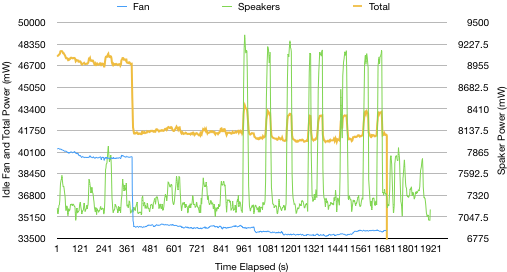
\includegraphics[width=1\textwidth]{figures/fanIdle.png}
  \caption{Idle Fan with figure \ref{fig:bestBballSum} trace.}
  \label{fig:fanIdle}
\end{figure}

\begin{figure}[H]
  \centering
  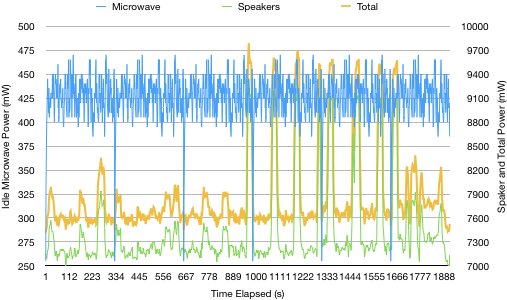
\includegraphics[width=1\textwidth]{figures/uWaveIdle.png}
  \caption{Idle microwave with figure \ref{fig:bestBballSum} trace.}
  \label{fig:uWaveIdle}
\end{figure}

\begin{figure}[H]
  \centering
  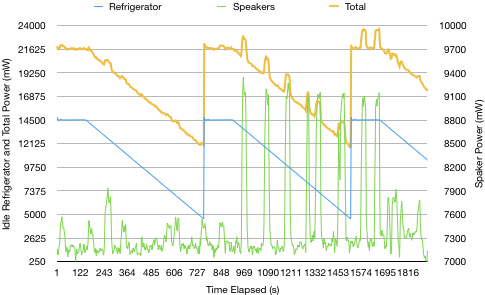
\includegraphics[width=1\textwidth]{figures/fridgeIdle.png}
  \caption{Idle refrigerator with figure \ref{fig:bestBballSum} trace.}
  \label{fig:fridgeIdle}
\end{figure}

\begin{figure}[H]
  \centering
  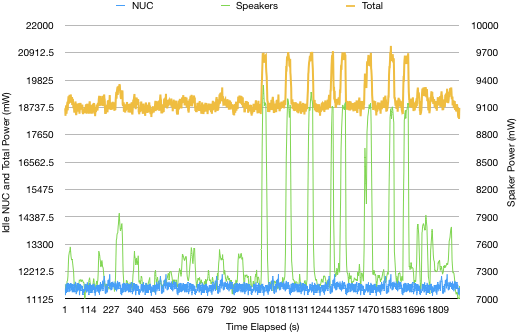
\includegraphics[width=1\textwidth]{figures/nucIdle.png}
  \caption{Idle PC (Intel NUC) with figure \ref{fig:bestBballSum} trace.}
  \label{fig:nucIdle}
\end{figure}

\begin{figure}[H]
  \centering
  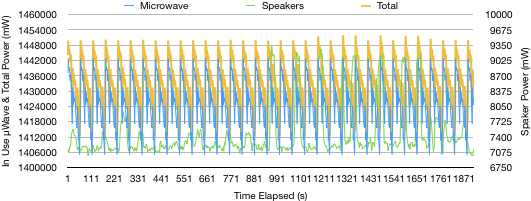
\includegraphics[width=1\textwidth]{figures/uWaveInUse.png}
  \caption{In use Microwave with figure \ref{fig:bestBballSum} trace.}
  \label{fig:uWaveInUse}
\end{figure}

\begin{figure}[H]
  \centering
  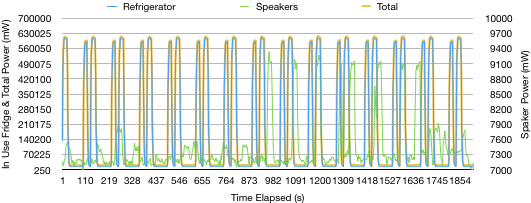
\includegraphics[width=1\textwidth]{figures/fridgeInUse.png}
  \caption{Fridge in the middle of cooling with figure \ref{fig:bestBballSum} trace.}
  \label{fig:fridgeInUse}
\end{figure}

\begin{figure}[H]
  \centering
  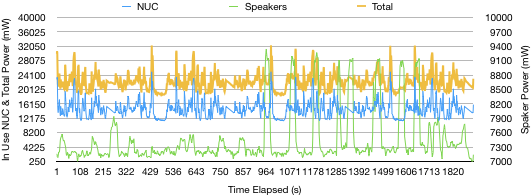
\includegraphics[width=1\textwidth]{figures/nucInUse.png}
  \caption{PC in use with figure \ref{fig:bestBballSum} trace.}
  \label{fig:nucInUse}
\end{figure}

\section{Smart Speaker Comparison}
\label{smartSpeakerComparisonSection}
The figures in section \ref{sumPowerGraph} show that the Echo Dot uses a lot more energy than the other smart speakers. Because of that, we wanted to compare the energy and network usages of the three smart speakers individually so that we can determine trade-offs that they make.

In the graphs below, we display power and network traces for the echo dot 1, Eufy genie 1, and Google home. We used the same time frame as the graph in figure \ref{fig:bestBballSeperate} for the two graphs below. We removed the second Echo Dot and Eufy Genie for simplicity.

In the same time frame as the two graphs below, we also recorded the average power usage and throughput for the smart speakers. For average power, from greatest to least, we have the Echo Dot (1650 mW), Eufy Genie (1325 mW), Google Home (1175 mW). For average throughput, from greatest to least, we have the Eufy Genie (1743 bytes), Google Home (800 bytes), Echo Dot (325 bytes).

\begin{figure}[H]
  \centering
  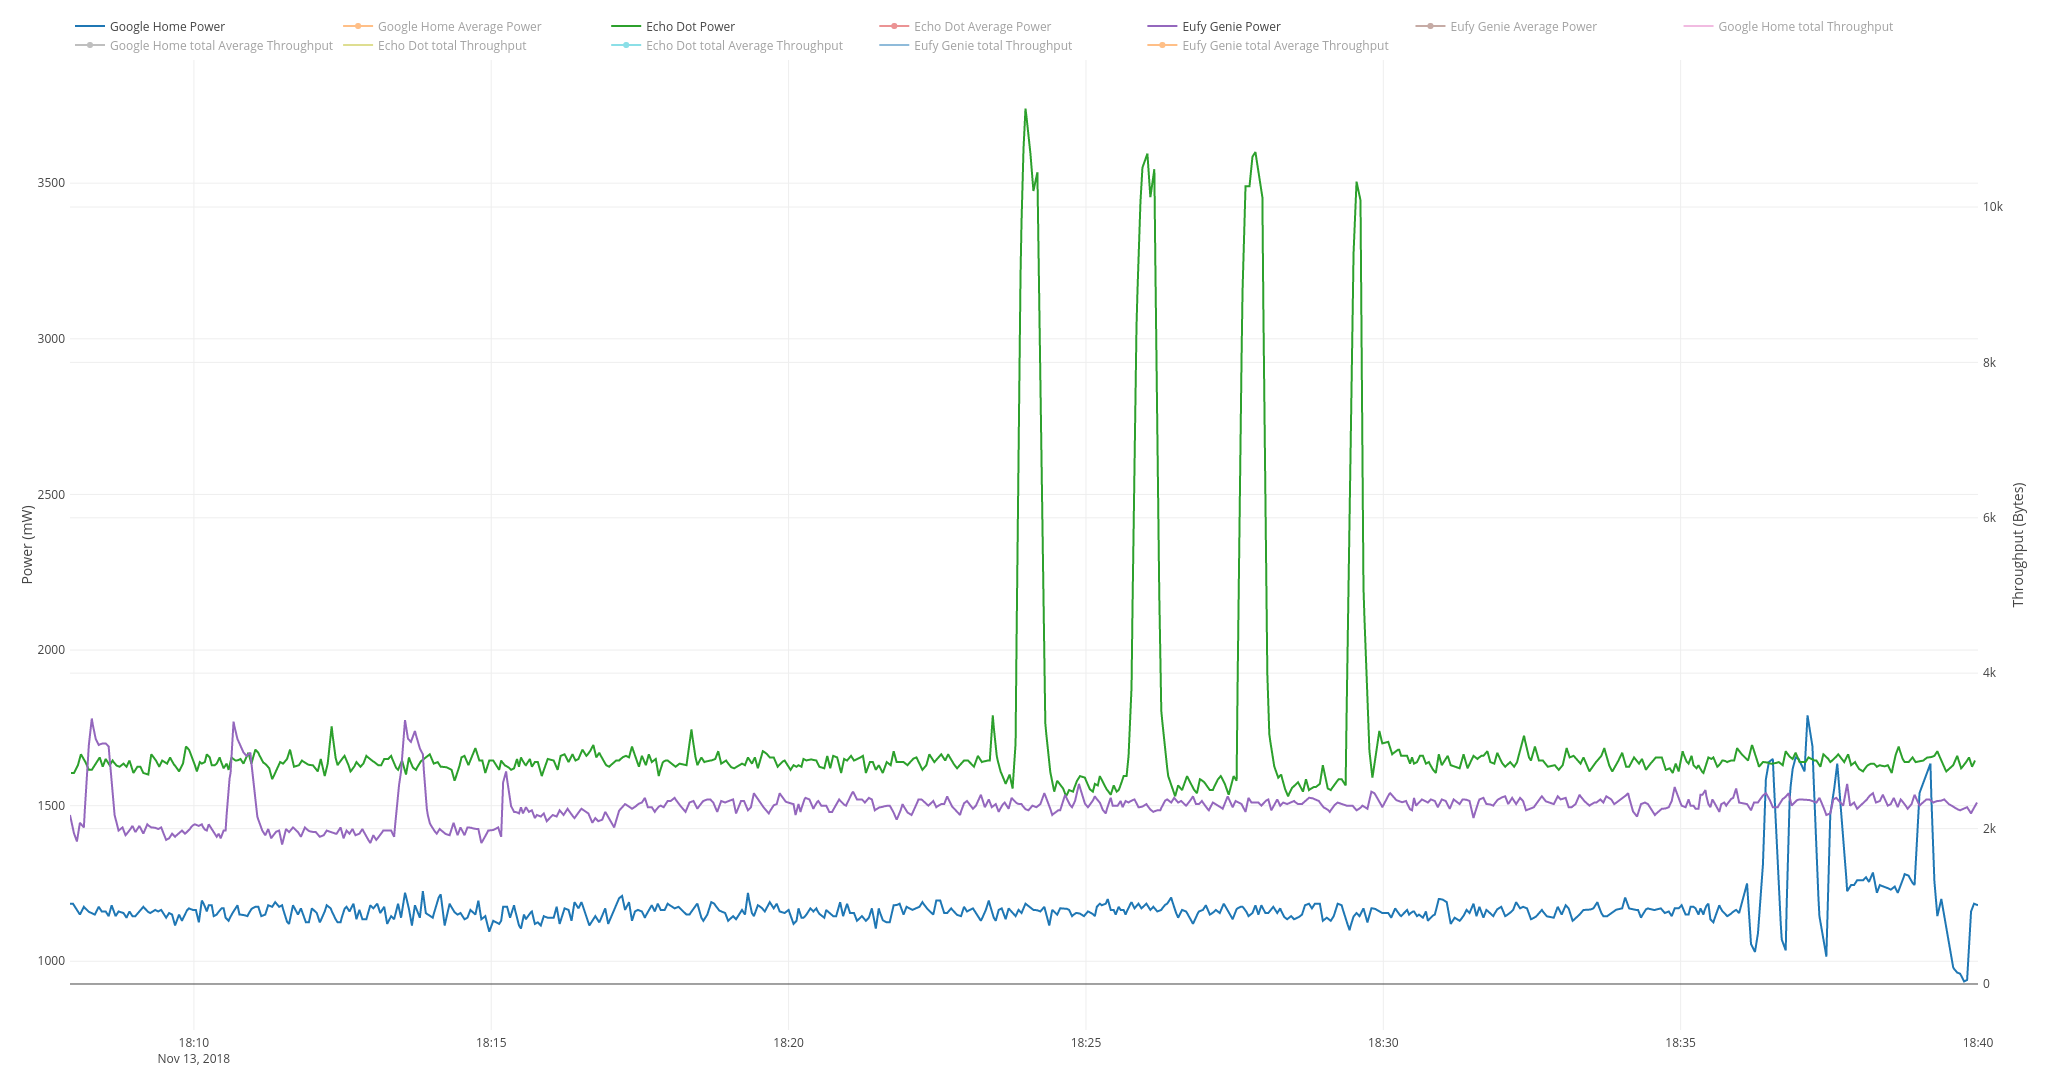
\includegraphics[width=1\textwidth]{figures/smartSpeakerSeperate.png}
  \caption{Power usage of Echo Dot 1, Eufy Genie 1, and Google Home over time when asked ``who is the best basketball player''. Same graph as figure \ref{fig:bestBballSeperate} with Echo DOt 2 and Eufy Genie removed.}
  \label{fig:smartSpeakerSeperate}
\end{figure}

\begin{figure}[H]
  \centering
  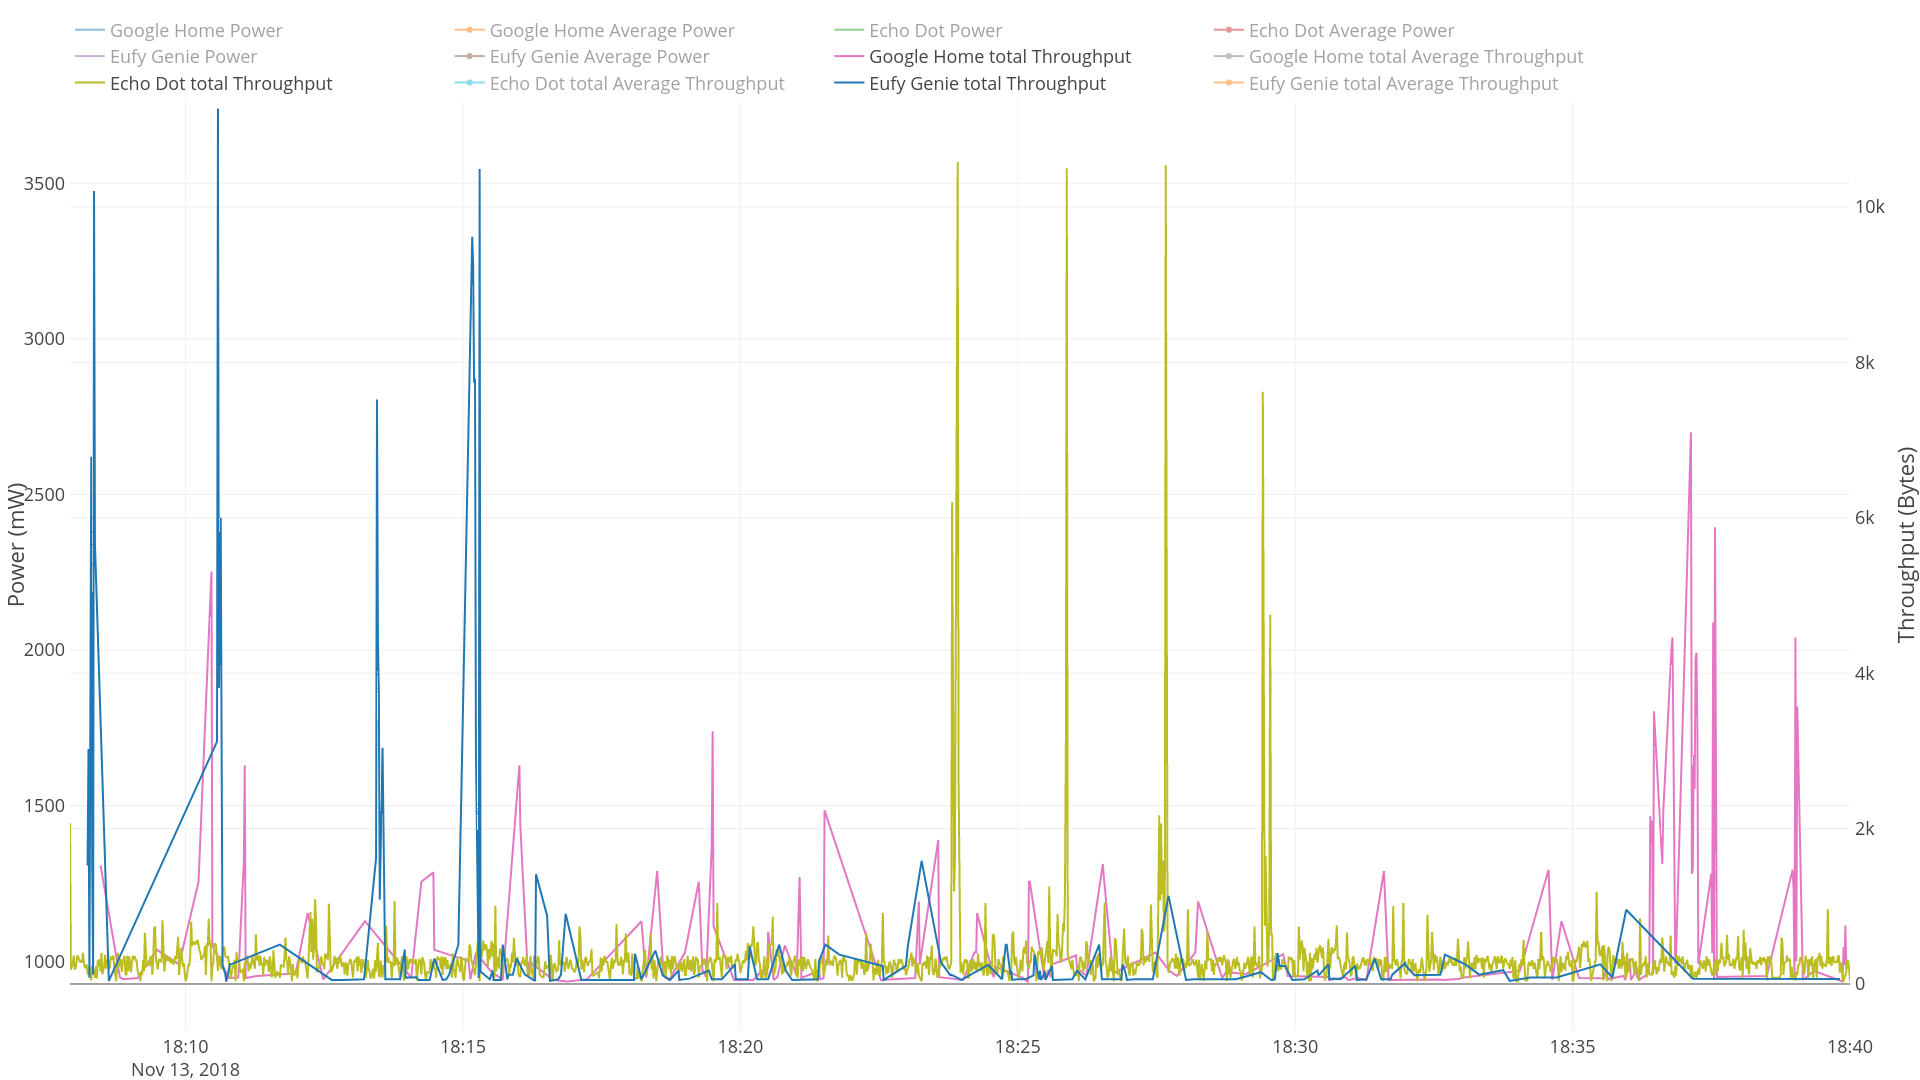
\includegraphics[width=1\textwidth]{figures/smartSpeakerNetworkSeperate.png}
  \caption{Power usage of Echo Dot 1, Eufy Genie 1, and Google Home over time when asked ``who is the best basketball player''. Same time frame as figure \ref{fig:smartSpeakerSeperate}}
  \label{fig:smartSpeakerNetworkSeperate}
\end{figure}
